\documentclass[10]{article}
%\documentclass[11pt]{book}
\usepackage{hyperref}
\usepackage{amsfonts,amssymb,amsmath,amsthm,cite}
\usepackage{graphicx}
\usepackage[toc,page]{appendix}
\usepackage{nicefrac}
%% \usepackage[francais]{babel}
\usepackage[applemac]{inputenc}
\usepackage{amssymb, euscript}
\usepackage[matrix,arrow,curve]{xy}
\usepackage{graphicx}
\usepackage{tabularx}
\usepackage{float}
\usepackage{tikz}
\usepackage{slashed}
\usepackage{mathrsfs}
\usepackage{multirow}

%\usepackage{mathtools}

\usetikzlibrary{matrix}

\usepackage[T1]{fontenc}
\usepackage{amsfonts,cite}
\usepackage{graphicx}

%% \usepackage[francais]{babel}
\usepackage[applemac]{inputenc}


\usepackage[sc]{mathpazo}
\usepackage{environ}

\linespread{1.05}         % Palatino needs more leading (space between lines)


%\usepackage[usenames]{color}



\DeclareFontFamily{T1}{pzc}{}
\DeclareFontShape{T1}{pzc}{m}{it}{1.8 <-> pzcmi8t}{}
\DeclareMathAlphabet{\mathpzc}{T1}{pzc}{m}{it}
% the command for it is \mathpzc

\textwidth=140mm


% % % % % % % % % % % % % % % % % % % %
\theoremstyle{plain}
\newtheorem{prop}{Proposition}[section]
\newtheorem{prdf}[prop]{Proposition and Definition}
\newtheorem{lem}[prop]{Lemma}%[section]
\newtheorem{cor}[prop]{Corollary}%[section]
\newtheorem{thm}[prop]{Theorem}%[section]
\newtheorem{theorem}[prop]{Theorem}
\newtheorem{lemma}[prop]{Lemma}
\newtheorem{proposition}[prop]{Proposition}
\newtheorem{corollary}[prop]{Corollary}
\newtheorem{statement}[prop]{Statement}

\theoremstyle{definition}
\newtheorem{defn}[prop]{Definition}%[section]
\newtheorem{cordefn}[prop]{Corollary and Definition}%[section]
\newtheorem{empt}[prop]{}%[section]
\newtheorem{exm}[prop]{Example}%[section]
\newtheorem{rem}[prop]{Remark}%[section]
\newtheorem{prob}[prop]{Problem}
\newtheorem{conj}{Conjecture}       %% Hypothesis 1
\newtheorem{cond}{Condition}        %% Condition 1
%\newtheorem{axiom}[thm]{Axiom}           %% Axiom 1 modified
\newtheorem{fact}[prop]{Fact}
\newtheorem{ques}{Question}         %% Question 1
\newtheorem{answ}{Answer}           %% Answer 1
\newtheorem{notn}{Notation}        %% Notations are not numbered

\theoremstyle{definition}
\newtheorem{notation}[prop]{Notation}
\newtheorem{definition}[prop]{Definition}
\newtheorem{example}[prop]{Example}
\newtheorem{exercise}[prop]{Exercise}
\newtheorem{conclusion}[prop]{Conclusion}
\newtheorem{conjecture}[prop]{Conjecture}
\newtheorem{criterion}[prop]{Criterion}
\newtheorem{summary}[prop]{Summary}
\newtheorem{axiom}[prop]{Axiom}
\newtheorem{problem}[prop]{Problem}
%\theoremstyle{remark}
\newtheorem{remark}[prop]{Remark}

\numberwithin{equation}{section}
\newtheorem*{claim}{Claim}
\DeclareMathOperator{\Dom}{Dom}              %% domain of an operator
\newcommand{\Dslash}{{D\mkern-11.5mu/\,}}    %% Dirac operator


%\newcommand\myeq{\stackrel{\mathclap{\normalfont\mbox{def}}}{=}}
\newcommand{\nor}[1]{\left\Vert #1\right\Vert}    %\nor{x}=||x||
\newcommand{\vertiii}[1]{{\left\vert\kern-0.25ex\left\vert\kern-0.25ex\left\vert #1
		\right\vert\kern-0.25ex\right\vert\kern-0.25ex\right\vert}}
\newcommand{\Ga}{\Gamma}  
\newcommand{\coker}{\mathrm{coker}}                   %% short for  \Gamma
\newcommand{\Coo}{C^\infty}                  %% smooth functions
% % % % % % % % % % % % % % % % % % % %


\usepackage[sc]{mathpazo}
\linespread{1.05}         % Palatino needs more leading (space between lines)

\newbox\ncintdbox \newbox\ncinttbox %% noncommutative integral symbols
\setbox0=\hbox{$-$} \setbox2=\hbox{$\displaystyle\int$}
\setbox\ncintdbox=\hbox{\rlap{\hbox
		to \wd2{\hskip-.125em \box2\relax\hfil}}\box0\kern.1em}
\setbox0=\hbox{$\vcenter{\hrule width 4pt}$}
\setbox2=\hbox{$\textstyle\int$} \setbox\ncinttbox=\hbox{\rlap{\hbox
		to \wd2{\hskip-.175em \box2\relax\hfil}}\box0\kern.1em}

\newcommand{\ncint}{\mathop{\mathchoice{\copy\ncintdbox}%
		{\copy\ncinttbox}{\copy\ncinttbox}%
		{\copy\ncinttbox}}\nolimits}  %% NC integral

%%% Repeated relations:
\newcommand{\xyx}{\times\cdots\times}      %% repeated product
\newcommand{\opyop}{\oplus\cdots\oplus}    %% repeated direct sum
\newcommand{\oxyox}{\otimes\cdots\otimes}  %% repeated tensor product
\newcommand{\wyw}{\wedge\cdots\wedge}      %% repeated exterior product
\newcommand{\subysub}{\subset\hdots\subset}      %% repeated subset
\newcommand{\supysup}{\supset\hdots\supset}      %% repeated supset
\newcommand{\rep}{\mathfrak{rep}}
\newcommand{\lift}{\mathfrak{lift}}
\newcommand{\desc}{\mathfrak{desc}}
%%% Roman letters:
\newcommand{\id}{\mathrm{id}}                %% identity map
\newcommand{\Id}{\mathrm{Id}}                %% identity map
\newcommand{\pt}{\mathrm{pt}}                %% a point
\newcommand{\const}{\mathrm{const}}          %% a constant
\newcommand{\codim}{\mathrm{codim}}          %% codimension
\newcommand{\cyc}{\mathrm{cyclic}}  %% cyclic sum
\renewcommand{\d}{\mathrm{d}}       %% commutative differential
\newcommand{\dR}{\mathrm{dR}}       %% de~Rham cohomology
\newcommand{\proj}{\mathrm{proj}}                %% a projection



\newcommand*{\Mult}{\mathcal M}% multiplier algebra

\newcommand{\A}{\mathcal{A}}                 %%\newcommand{\unitsv}[1]{#1^{(0)}}
\newcommand{\units}{G^{(0)}}
\newcommand{\haars}{\{\lambda^{u}\}_{u\in\units}}
\newcommand{\shaars}{\{\lambda_{u}\}_{u\in\units}}
\newcommand{\haarsv}[2]{\{\lambda^{#2}_{#1}\}_{#2\in\unitsv{#1}}}
\newcommand{\haarv}[2]{\lambda^{#2}_{#1}}

\renewcommand{\a}{\alpha}                    %% short for  \alphapha
\DeclareMathOperator{\ad}{ad}                %% infml adjoint repn
\newcommand{\as}{\quad\mbox{as}\enspace}     %% `as' with spacing
\newcommand{\Aun}{\widetilde{\mathcal{A}}}   %% unital algebra
\newcommand{\B}{\mathcal{B}}                 %% space of distributions
\newcommand{\E}{\mathcal{E}}                 %% space of distributions
\renewcommand{\b}{\beta}                     %% short for \beta
\newcommand{\braCket}[3]{\langle#1\mathbin|#2\mathbin|#3\rangle}
\newcommand{\braket}[2]{\langle#1\mathbin|#2\rangle} %% <w|z>
\newcommand{\C}{\mathbb{C}}                  %% complex numbers
\newcommand{\CC}{\mathcal{C}}                %% space of distributions
\newcommand{\cc}{\mathbf{c}}                 %% Hochschild cycle
\DeclareMathOperator{\Cl}{C\ell}             %% Clifford algebra
\newcommand{\F}{\mathcal{F}}                 %% space of test functions
\newcommand{\G}{\mathcal{G}}                 %% 
\newcommand{\D}{\mathcal{D}}                 %% Moyal L^2-filtration
\renewcommand{\H}{\mathcal{H}}               %% Hilbert space
\newcommand{\half}{\tfrac{1}{2}}             %% small fraction  1/2
\newcommand{\hh}{\mathcal{H}}                %% Hilbert space
\newcommand{\hookto}{\hookrightarrow}        %% abbreviation
\newcommand{\Ht}{{\widetilde{\mathcal{H}}}}  %% Hilbert space of forms
\newcommand{\I}{\mathcal{I}}                 %% tracelike functions
\DeclareMathOperator{\Junk}{Junk}            %% the junk DGA ideal
\newcommand{\K}{\mathcal{K}}                 %% compact operators
\newcommand{\ket}[1]{|#1\rangle}             %% ket vector
\newcommand{\ketbra}[2]{|#1\rangle\langle#2|} %% rank one operator
\renewcommand{\L}{\mathcal{L}}               %% operator algebra
\newcommand{\La}{\Lambda}                    %% short for \Lambda
\newcommand{\la}{\lambda}                    %% short for \lambda
\newcommand{\lf}{L_f^\theta}                 %% left mult operator
\newcommand{\M}{\mathcal{M}}                 %% Moyal multplr algebra
\newcommand{\mm}{\mathcal{M}^\theta}
%\newcommand{{{\star_{\theta}}}{{\mathchoice{\mathbin{\;|\;ar_{_\theta}}}
			%            {\mathbin{\;|\;ar_{_\theta}}}           %% Moyal
			%            {{\;|\;ar_\theta}}{{\;|\;ar_\theta}}}}    %% product
	\newcommand{\N}{\mathbb{N}}                  %% nonnegative integers
	\newcommand{\NN}{\mathcal{N}}                %% a Moyal algebra
	\newcommand{\nb}{\nabla}                     %% gradient
	\newcommand{\Oh}{\mathcal{O}}                %% comm multiplier alg
	\newcommand{\om}{\omega}                     %% short for \omega
	\newcommand{\opp}{{\mathrm{op}}}             %% opposite algebra
	\newcommand{\ox}{\otimes}                    %% tensor product
	\newcommand{\eps}{\varepsilon}                    %% tensor product
	\newcommand{\otimesyox}{\otimes\cdots\otimes}    %% repeated tensor product
	\newcommand{\pa}{\partial}                   %% short for \partial
	\newcommand{\pd}[2]{\frac{\partial#1}{\partial#2}}%% partial derivative
	\newcommand{\piso}[1]{\lfloor#1\rfloor}      %% integer part
	\newcommand{\PsiDO}{\Psi~\mathrm{DO}}         %% pseudodiffl operators
	\newcommand{\Q}{\mathbb{Q}}                  %% rational numbers
	\newcommand{\R}{\mathbb{R}}                  %% real numbers
	\newcommand{\rdl}{R_\Dslash(\lambda)}        %% resolvent
	\newcommand{\roundbraket}[2]{(#1\mathbin|#2)} %% (w|z)
	\newcommand{\row}[3]{{#1}_{#2},\dots,{#1}_{#3}} %% list: a_1,...,a_n
	\newcommand{\sepword}[1]{\quad\mbox{#1}\quad} %% well-spaced words
	\newcommand{\set}[1]{\{\,#1\,\}}             %% set notation
	\newcommand{\Sf}{\mathbb{S}}                 %% sphere
	\newcommand{\uhor}[1]{\Omega^1_{hor}#1}
	\newcommand{\sco}[1]{{\sp{(#1)}}}
	\newcommand{\sw}[1]{{\sb{(#1)}}}
	\DeclareMathOperator{\spec}{sp}              %% spectrum
	\renewcommand{\SS}{\mathcal{S}}              %% Schwartz space
	\newcommand{\sss}{\mathcal{S}}               %% Schwartz space
	\DeclareMathOperator{\supp}{\mathfrak{supp}}            %% support
	\newcommand{\T}{\mathbb{T}}                  %% circle as a group
	\renewcommand{\th}{\theta}                   %% short for \theta
	\newcommand{\thalf}{\tfrac{1}{2}}            %% small* fraction 1/2
	\newcommand{\tihalf}{\tfrac{i}{2}}           %% small* fraction i/2
	\newcommand{\tpi}{{\tilde\pi}}               %% extended representation
	\DeclareMathOperator{\Tr}{Tr}                %% trace of operator
	\DeclareMathOperator{\tr}{tr}                %% trace of matrix
	\newcommand{\del}{\partial}                  %% short for  \partial
	\DeclareMathOperator{\tsum}{{\textstyle\sum}} %% small sum in display
	\newcommand{\V}{\mathcal{V}}                 %% test function space
	\newcommand{\vac}{\ket{0}}                   %% vacuum ket vector
	\newcommand{\vf}{\varphi}                    %% scalar field
	\newcommand{\w}{\wedge}                      %% exterior product
	\DeclareMathOperator{\wres}{wres}            %% density of Wresidue
	\newcommand{\x}{\times}                      %% cross
	\newcommand{\Z}{\mathbb{Z}}                  %% integers
	\newcommand{\7}{\dagger}                     %% short for + symbol
	\newcommand{\8}{\bullet}                     %% anonymous degree
	\renewcommand{\.}{\cdot}                     %% anonymous variable
	\renewcommand{\:}{\colon}                    %% colon in  f: A -> B
	
	%\newcommand{\sA}{\mathscr{A}}       %%
	\newcommand{\sA}{\mathcal{A}} 
	\newcommand{\sB}{\mathcal{B}}       %%
	\newcommand{\sC}{\mathcal{C}}       %%
	\newcommand{\sD}{\mathcal{D}}       %%
	\newcommand{\sE}{\mathcal{E}}       %%
	\newcommand{\sF}{\mathcal{F}}       %%
	\newcommand{\sG}{\mathcal{G}}       %%
	\newcommand{\sH}{\mathcal{H}}       %%
	\newcommand{\sI}{\mathcal{I}}       %%
	\newcommand{\sJ}{\mathcal{J}}       %%
	\newcommand{\sK}{\mathcal{K}}       %%
	\newcommand{\sL}{\mathcal{L}}       %%
	\newcommand{\sM}{\mathcal{M}}       %%
	\newcommand{\sN}{\mathcal{N}}       %%
	\newcommand{\sO}{\mathcal{O}}       %%
	\newcommand{\sP}{\mathcal{P}}       %%
	\newcommand{\sQ}{\mathcal{Q}}       %%
	\newcommand{\sR}{\mathcal{R}}       %%
	\newcommand{\sS}{\mathcal{S}}       %%
	\newcommand{\sT}{\mathcal{T}}       %%
	\newcommand{\sU}{\mathcal{U}}       %%
	\newcommand{\sV}{\mathcal{V}}       %%
	\newcommand{\sX}{\mathcal{X}}       %%
	\newcommand{\sY}{\mathcal{Y}}       %%
	\newcommand{\sZ}{\mathcal{Z}}       %%
	
	\newcommand{\Om}{\Omega}       %%
	
	
	\DeclareMathOperator{\ptr}{ptr}     %% Poisson trace
	\DeclareMathOperator{\Trw}{Tr_\omega} %% Dixmier trace
	\DeclareMathOperator{\vol}{Vol}     %% total volume
	\DeclareMathOperator{\Vol}{Vol}     %% total volume
	\DeclareMathOperator{\Area}{Area}   %% area of a surface
	\DeclareMathOperator{\Wres}{Wres}   %% (Wodzicki) residue
	
	\newcommand{\dd}[1]{\frac{\partial}{\partial#1}}   %% partial derivation
	\newcommand{\ddt}[1]{\frac{d}{d#1}}                %% derivative
	\newcommand{\inv}[1]{\frac{1}{#1}}                 %% inverse
	\newcommand{\sfrac}[2]{{\scriptstyle\frac{#1}{#2}}} %% tiny fraction
	
	\newcommand{\bA}{\mathbb{A}}       %%
	\newcommand{\bB}{\mathbb{B}}       %%
	\newcommand{\bC}{\mathbb{C}}       %%
	\newcommand{\bCP}{\mathbb{C}P}     %%
	\newcommand{\bD}{\mathbb{D}}       %%
	\newcommand{\bE}{\mathbb{E}}       %%
	\newcommand{\bF}{\mathbb{F}}       %%
	\newcommand{\bG}{\mathbb{G}}       %%
	\newcommand{\bH}{\mathbb{H}}       %%
	\newcommand{\bHP}{\mathbb{H}P}     %%
	\newcommand{\bI}{\mathbb{I}}       %%
	\newcommand{\bJ}{\mathbb{J}}       %%
	\newcommand{\bK}{\mathbb{K}}       %%
	\newcommand{\bL}{\mathbb{L}}       %%
	\newcommand{\bM}{\mathbb{M}}       %%
	\newcommand{\bN}{\mathbb{N}}       %%
	\newcommand{\bO}{\mathbb{O}}       %%
	\newcommand{\bOP}{\mathbb{O}P}     %%
	\newcommand{\bP}{\mathbb{P}}       %%
	\newcommand{\bQ}{\mathbb{Q}}       %%
	\newcommand{\bR}{\mathbb{R}}       %%
	\newcommand{\bRP}{\mathbb{R}P}     %%
	\newcommand{\bS}{\mathbb{S}}       %%
	\newcommand{\bT}{\mathbb{T}}       %%
	\newcommand{\bU}{\mathbb{U}}       %%
	\newcommand{\bV}{\mathbb{V}}       %%
	\newcommand{\bX}{\mathbb{X}}       %%
	\newcommand{\bY}{\mathbb{Y}}       %%
	\newcommand{\bZ}{\mathbb{Z}}       %%
	
	\newcommand{\bydef}{\stackrel{\mathrm{def}}{=}}          %% 
	
	
	\newcommand{\al}{\alpha}          %% short for  \alpha
	\newcommand{\bt}{\beta}           %% short for  \beta
	\newcommand{\Dl}{\Delta}          %% short for  \Delta
	\newcommand{\dl}{\delta}          %% short for  \delta
	\newcommand{\ga}{\gamma}          %% short for  \gamma
	\newcommand{\ka}{\kappa}          %% short for  \kappa
	\newcommand{\sg}{\sigma}          %% short for  \sigma
	\newcommand{\Sg}{\Sigma}          %% short for  \Sigma
	\newcommand{\Th}{\Theta}          %% short for  \Theta
	\renewcommand{\th}{\theta}        %% short for  \theta
	\newcommand{\vth}{\vartheta}      %% short for  \vartheta
	\newcommand{\ze}{\zeta}           %% short for  \zeta
	
	\DeclareMathOperator{\ord}{ord}     %% order of a PsiDO
	\DeclareMathOperator{\rank}{rank}   %% rank of a vector bundle
	\DeclareMathOperator{\sign}{sign}   %%
	\DeclareMathOperator{\sgn}{sgn}   %%
	\DeclareMathOperator{\chr}{char}   %%
	\DeclareMathOperator{\ev}{ev}       %% evaluation
	
	
	\newcommand{\Op}{\mathbf{Op}}
	\newcommand{\As}{\mathbf{As}}
	\newcommand{\Com}{\mathbf{Com}}
	\newcommand{\LLie}{\mathbf{Lie}}
	\newcommand{\Leib}{\mathbf{Leib}}
	\newcommand{\Zinb}{\mathbf{Zinb}}
	\newcommand{\Poiss}{\mathbf{Poiss}}
	
	\newcommand{\gX}{\mathfrak{X}}      %% vector fields
	\newcommand{\sol}{\mathfrak{so}}    %% special orthogonal Lie algebra
	\newcommand{\gm}{\mathfrak{m}}      %% maximal ideal
	
	
	\DeclareMathOperator{\Res}{Res}
	\DeclareMathOperator{\NCRes}{NCRes}
	\DeclareMathOperator{\Ind}{Ind}
	%% co/homology theories
	\DeclareMathOperator{\rH}{H}        %% any co/homology
	\DeclareMathOperator{\rC}{C}        %%  any co/chains
	\DeclareMathOperator{\rZ}{Z}        %% cycles
	\DeclareMathOperator{\rB}{B}        %% boundaries
	\DeclareMathOperator{\rF}{F}        %% filtration
	\DeclareMathOperator{\Gr}{gr}        %% associated graded object
	\DeclareMathOperator{\rHc}{H_{\mathrm{c}}}   %% co/homology with compact support
	\DeclareMathOperator{\drH}{H_{\mathrm{dR}}}  %% de Rham co/homology
	\DeclareMathOperator{\cechH}{\check{H}}    %% Cech co/homology
	\DeclareMathOperator{\rK}{K}        %% K-groups
	\DeclareMathOperator{\rKO}{KO}        %% real K-groups
	\DeclareMathOperator{\rKU}{KU}        %% unitary K-groups
	\DeclareMathOperator{\rKSp}{KSp}        %% symplectic K-groups
	\DeclareMathOperator{\rR}{R}        %% representation ring
	\DeclareMathOperator{\rI}{I}        %% augmentation ideal
	\DeclareMathOperator{\HH}{HH}       %% Hochschild co/homology
	\DeclareMathOperator{\HC}{HC}       %% cyclic co/homology
	\DeclareMathOperator{\HP}{HP}       %% periodic cyclic co/homology
	\DeclareMathOperator{\HN}{HN}       %% negative cyclic co/homology
	\DeclareMathOperator{\HL}{HL}       %% Leibniz co/homology
	\DeclareMathOperator{\KK}{KK}       %% KK-theory
	\DeclareMathOperator{\KKK}{\mathbf{KK}}       %% KK-theory as a category
	\DeclareMathOperator{\Ell}{Ell}       %% Abstract elliptic operators
	\DeclareMathOperator{\cd}{cd}       %% cohomological dimension
	\DeclareMathOperator{\spn}{span}       %% span
	\DeclareMathOperator{\linspan}{span} %% linear span (can't use \span)
	\newcommand{\blank}{-}   
	
	
	
	\newcommand{\twobytwo}[4]{\begin{pmatrix} #1 & #2 \\ #3 & #4 \end{pmatrix}}
	\newcommand{\CGq}[6]{C_q\!\begin{pmatrix}#1&#2&#3\\#4&#5&#6\end{pmatrix}}
	%% q-Clebsch--Gordan coefficients
	\newcommand{\cz}{{\bullet}}         %% anonymous degree
	\newcommand{\nic}{{\vphantom{\dagger}}} %% invisible dagger
	\newcommand{\ep}{{\dagger}}         %% abbreviation for + symbol
	\newcommand{\downto}{\downarrow}    %% right hand limit
	\newcommand{\isom}{\cong}          %% isomorphism
	\newcommand{\lt}{\triangleright}    %% a left action
	\newcommand{\otto}{\leftrightarrow} %% bijection
	\newcommand{\rt}{\triangleleft}     %% a right action
	\newcommand{\semi}{\rtimes}         %% crossed product
	\newcommand{\tensor}{\otimes}       %% tensor product
	\newcommand{\cotensor}{\square}       %% cotensor product
	\newcommand{\trans}{\pitchfork}     %% transverse
	\newcommand{\ul}{\underline}        %% for sheaves
	\newcommand{\upto}{\uparrow}        %% left hand limit
	\renewcommand{\:}{\colon}           %% colon in  f: A -> B
	\newcommand{\blt}{\ast}
	\newcommand{\Co}{C_{\bullet}}
	\newcommand{\cCo}{C^{\bullet}}
	\newcommand{\nbs}{\nabla^S}         %% spin connection
	\newcommand{\up}{{\mathord{\uparrow}}} %% `up' spinors
	\newcommand{\dn}{{\mathord{\downarrow}}} %% `down' spinors
	\newcommand{\updn}{{\mathord{\updownarrow}}} %% up or down
	
	%%% Bilinear enclosures:
	
	\newcommand{\bbraket}[2]{\langle\!\langle#1\stroke#2\rangle\!\rangle}
	%% <<w|z>>
	\newcommand{\bracket}[2]{\langle#1,\, #2\rangle} %% <w,z>
	\newcommand{\scalar}[2]{\langle#1,\,#2\rangle} %% <w,z>
	\newcommand{\poiss}[2]{\{#1,\,#2\}} %% {w,z}
	\newcommand{\dst}[2]{\langle#1,#2\rangle} %% distributions <u,\phi>
	\newcommand{\pairing}[2]{(#1\stroke #2)} %% right-linear pairing
	\def\<#1|#2>{\langle#1\stroke#2\rangle} %% \braket (Dirac notation)
	\def\?#1|#2?{\{#1\stroke#2\}}        %% left-linear pairing
	
	%%% Accent-like macros:
	
	\renewcommand{\Bar}[1]{\overline{#1}} %% closure operator
	\renewcommand{\Hat}[1]{\widehat{#1}}  %% short for \widehat
	\renewcommand{\Tilde}[1]{\widetilde{#1}} %% short for \widetilde
	
	
	\DeclareMathOperator{\bCl}{\bC l}   %% complex Clifford algebra
	
	%%% Small fractions in displays:
	
	\newcommand{\ihalf}{\tfrac{i}{2}}   %% small fraction  i/2
	\newcommand{\quarter}{\tfrac{1}{4}} %% small fraction  1/4
	\newcommand{\shalf}{{\scriptstyle\frac{1}{2}}}  %% tiny fraction  1/2
	\newcommand{\third}{\tfrac{1}{3}}   %% small fraction  1/3
	\newcommand{\ssesq}{{\scriptstyle\frac{3}{2}}} %% tiny fraction  3/2
	\newcommand{\sesq}{{\mathchoice{\tsesq}{\tsesq}{\ssesq}{\ssesq}}} %% 3/2
	\newcommand{\tsesq}{\tfrac{3}{2}}   %% small fraction  3/2
	
	
	%\newcommand\eqdef{\overset{\mathclap{\normalfont\mbox{def}}}{=}}
	\newcommand\eqdef{\overset{\mathrm{def}}{=}}
	
	
	%+++++++++++++++++++++++++++++++++++
	
	\newcommand{\word}[1]{\quad\text{#1}\enspace} %% well-spaced words
	\newcommand{\words}[1]{\quad\text{#1}\quad} %% better-spaced words
	\newcommand{\su}[1]{{\sp{[#1]}}}
	
	\def\<#1,#2>{\langle#1,#2\rangle}            %% bilinear pairing
	\def\ee_#1{e_{{\scriptscriptstyle#1}}}       %% basis projector
	\def\wick:#1:{\mathopen:#1\mathclose:}       %% Wick-ordered operator
	
	\newcommand{\opname}[1]{\mathop{\mathrm{#1}}\nolimits}
	
	\newcommand{\hideqed}{\renewcommand{\qed}{}} %% to suppress `\qed'
	
	
	%%%%%%%%%%%%%%%%%%%%%%%%%%%%%
	%% 2. Some internal machinery
	%%%%%%%%%%%%%%%%%%%%%%%%%%%%%
	
	\newbox\ncintdbox \newbox\ncinttbox %% noncommutative integral symbols
	\setbox0=\hbox{$-$}
	\setbox2=\hbox{$\displaystyle\int$}
	\setbox\ncintdbox=\hbox{\rlap{\hbox
			to \wd2{\box2\relax\hfil}}\box0\kern.1em}
	\setbox0=\hbox{$\vcenter{\hrule width 4pt}$}
	\setbox2=\hbox{$\textstyle\int$}
	\setbox\ncinttbox=\hbox{\rlap{\hbox
			to \wd2{\hskip-.05em\box2\relax\hfil}}\box0\kern.1em}
	
	\newcommand{\disp}{\displaystyle} %% short for  \displaystyle
	
	%\newcommand{\hideqed}{\renewcommand{\qed}{}} %% no `\qed' at end-proof
	
	\newcommand{\stroke}{\mathbin|}   %% (for `\bbraket' and such)
	\newcommand{\tribar}{|\mkern-2mu|\mkern-2mu|} %% norm bars: |||
	
	%%% Enclose one argument with delimiters:
	
	\newcommand{\bra}[1]{\langle{#1}\rvert} %% bra vector <w|
	\newcommand{\kett}[1]{\lvert#1\rangle\!\rangle} %% ket 2-vector |y>>
	\newcommand{\snorm}[1]{\mathopen{\tribar}{#1}%
		\mathclose{\tribar}}                 %% norm |||x|||
	
	
	\newcommand{\End}{\mathrm{End}}       %%
	\newcommand{\Ext}{\mathrm{Ext}}       %%
	\newcommand{\Hom}{\mathrm{Hom}}       %%
	\newcommand{\Mrt}{\mathrm{Mrt}}       %%
	\newcommand{\grad}{\mathrm{grad}}       %%
	\newcommand{\Spin}{\mathrm{Spin}}       %%
	\newcommand{\Ad}{\mathrm{Ad}}       %%
	\newcommand{\Pic}{\mathrm{Pic}}       %%
	\newcommand{\Aut}{\mathrm{Aut}}       %%
	\newcommand{\Inn}{\mathrm{Inn}}       %%
	\newcommand{\Out}{\mathrm{Out}}       %%
	\newcommand{\Homeo}{\mathrm{Homeo}}       %%
	\newcommand{\Diff}{\mathrm{Diff}}       %%
	\newcommand{\im}{\mathrm{im}}       %%
	
	
	\newcommand{\SO}{\mathrm{SO}}       %%
	\newcommand{\SU}{SU}       %%
	\newcommand{\gso}{\mathfrak{so}}    %% special orthogonal Lie algebra
	\newcommand{\gero}{\mathfrak{o}}    %% orthogonal Lie algebra
	\newcommand{\gspin}{\mathfrak{spin}} %% spin Lie algebra
	\newcommand{\gu}{\mathfrak{u}}      %% unitary Lie algebra
	\newcommand{\gsu}{\mathfrak{su}}    %% special unitary Lie algebra
	\newcommand{\gsl}{\mathfrak{sl}}    %% special linear Lie algebra
	\newcommand{\gsp}{\mathfrak{sp}}    %% symplectic linear Lie algebra
	
	%\newcommand{\bes}{\begin{equation}\begin{split}}
			%\newcommand{\ees}{\end{split}\end{equation}}
	%\NewEnviron{split.enviro}{%
		%	\begin{equation}\begin{split}
				%	\BODY
				%	\end{split}\end{equation}
		%$}
	\newenvironment{splitequation}{\begin{equation}\begin{split}}{\end{split}\end{equation}}
	
	%Begin equation split: Begin equation split = bes
	\newcommand{\bs}{\begin{split}}
		\newcommand{\es}{\end{split}}
	\newcommand{\be}{\begin{equation}}
		\renewcommand{\ee}{\end{equation}}
	\newcommand{\bea}{\begin{eqnarray}}
		\newcommand{\eea}{\end{eqnarray}}
	\newcommand{\bean}{\begin{eqnarray*}}
		\newcommand{\eean}{\end{eqnarray*}}
	\newcommand{\brray}{\begin{array}}
		\newcommand{\erray}{\end{array}}
	\newenvironment{equations}
	{\begin{equation}
			\begin{split}}
			{\end{split}
	\end{equation}}
	\newcommand{\Hsquare}{%
		\text{\fboxsep=-.2pt\fbox{\rule{0pt}{1ex}\rule{1ex}{0pt}}}%
	}
	
	\title{Grothendieck $C^*$-algebras and their cohomology}
	
	\author
	{\textbf{Petr R. Ivankov*}\\
		e-mail: * monster.ivankov@gmail.com \\
	}
	
	\begin{document}

\maketitle  %\setlength{\parindent}{0pt}
\pagestyle{plain}


%\vspace{1 in}


%\noindent




%\end{abstract}


\section{General theory}

Let $A$ be a $C^*$-algebra. We define a category $\mathbf{Hered}/A$ such that
\begin{itemize}
	\item $\mathbf{Hered}/A$-objects are hereditary $C^*$- subalgebras of $A$.
	\item $\mathbf{Hered}/A$-morphism  from $B' \hookto A$ to $B'' \hookto A$ is an inclusion $B'\subset B''$ such that a following diagram 
				\newline
	\begin{tikzpicture}
		\matrix (m) [matrix of math nodes,row sep=3em,column sep=4em,minimum width=2em]
		{
			B'  &  & B''\\ 
			& A &\\};
		\path[-stealth]
		(m-1-1) edge node [above] {} (m-1-3)
		(m-1-1) edge node [above]  {} (m-2-2)
		(m-1-3) edge node [right]  {} (m-2-2);
	\end{tikzpicture}
\\
is commutative.
\end{itemize}
For any two $\mathbf{Hered}/A$-objects $B', B''$ we define their \textit{fibre product} (cf. Definition \ref{pullback_defn}) by the following way
$$
B'\times_A B'' \bydef B'\cap B''.
$$
For any $\mathbf{Hered}/A$-object a distinguished set of families of maps $\left\{B_\iota \hookto B\right\}_{\iota\in I}$, called a \textit{covering} of $B$, 
satisfying the following axioms: 

\begin{exercise}
Prove that a described above system of coverings satisfy to the conditions (b) and (c) of the Definition \ref{site_defn}.
\end{exercise}

\begin{definition}
We say that $A$ is a \textit{Grothendieck $C^*$-algebra} if a described above system of coverings satisfy to the condition (a) of the Definition  \ref{site_defn}. Any {Grothendieck $C^*$-algebra} naturally yields a Grothendieck topology which is said to be $A$-\textit{topology}.
\end{definition}
\begin{exercise}
 For any locally compact Hausdorff space $\sX$ an algebra $C_0\left(\sX \right)$ is a {Grothendieck $C^*$-algebra} 	and $C_0\left(\sX\right)$-topology  is naturally isomorphic to a classical topology of $\sX$.
\end{exercise}


\begin{appendices}
	\section{Categories and functors}
	
	\subsection{Categories and limits}
	\begin{definition}\label{category_defn}\cite{goldblatt:topoi}
	%	Axiomatic Definition of a Category. 
	A \textit{category} $\mathscr C$ comprises 
	\begin{itemize}
		\item[(1)] 	 a collection of things called $\mathscr C$-\textit{objects}; 
	\item[(2)] a collection of things called $\mathscr C$-\textit{arrows}  or $\mathscr C$-\textit{morphisms}; 
	\item[(3)] operations assigning to each  $\mathscr C$-arrow $f$  $\mathscr C$-object $\mathrm{dom}f$ (the 
		"domain" of $f$) and a $\mathscr C$-object $\mathrm{cod}f$ (the "codomain" of $f$). If $a =\mathrm{dom} f$  
		and $b =\mathrm{cod} f$ we display this as 
		\bean
		f: a \to b\quad \text{or}\quad  a \xrightarrow{f} b;
		\eean
		\item[(4)] an operation assigning to each pair $\left(g, f\right)$ of $\mathscr C$-arrows with $\mathrm{dom}g = \mathrm{cod} f$.
		 A $\mathscr{C}$-arrow  $g\circ f$, the \textit{composite of f and g}, having $\mathrm{dom}g\circ f= \mathrm{dom}f$ and  $\mathrm{cod }g\circ f= \mathrm{cod}g$, i.e. $g\circ f:  \mathrm{dom}f \to \mathrm{cod}g$  such that the following condition obtains:
		 
		 \textit{	Associative Law}: Given the configuration 
		$$
		a \xrightarrow{f}	b \xrightarrow{g}	c \xrightarrow{h}d
		$$ 
		of  $\mathscr{C}$-objects and $\mathscr{C}$-arrows  then $h \circ \left(g \circ f\right)= \left(h \circ g\right)\circ f$;
				\item[(5)] an assignment to each $\mathscr{C}$-object $b$ of a $\mathscr{C}$-arrow $\mathbb{1}_b : b \to b$, called the \textit{identity arrow} on $b$, such that 
				
				\textit{Identity Law}: For any $\mathscr{C}$-arrows $f: a \to b$ and $g : b \to c$ one has
				\bean
				\mathbb{1}_b \circ f = f \quad \text{and}\quad g\circ \mathbb{1}_b= g.
				\eean
		\end{itemize}

	\end{definition}

\begin{notation}\label{category_not}
If $a, b$ are  $\mathscr{C}$-objects then we denote by  $\mathscr{C}\left(a, b \right)$  a family of all arrows from $a$ to $b$.
\end{notation}
	\begin{definition}\label{dual_cat_defn}\cite{goldblatt:topoi}
	If  $\mathscr C$ is a category then its \textit{dual} or \textit{opposite} category $\mathscr C^{\mathrm{op}}$ is constructed as follows: 
	\begin{itemize}
		\item $\mathscr C$ and $\mathscr C^{\mathrm{op}}$ have the same objects.
		\item For each arrow $f: a\to b$ o we 
		introduce an arrow  $f^{\mathrm{op}}: b\to a$ in $\mathscr C^{\mathrm{op}}$, these being all and only the arrows.
		\item  The composite $f^{\mathrm{op}}\circ g^{\mathrm{op}}$ is defined precisely when $g\circ f$ is defined in $\mathscr C$
		and has $f\circ g\bydef \left(g\circ f \right)^{\mathrm{op}}$.
	\end{itemize}
	
\end{definition}
\begin{definition}\label{init_ob_defn}\cite{goldblatt:topoi}
	An object $0$ is \textit{initial} in a category $\mathscr C$ if for every $\mathscr C$-object $a$ there is one and only one arrow from $0$ to $a$ in $\mathscr C$.
\end{definition}
\begin{definition}\label{term_ob_defn}\cite{goldblatt:topoi}
	An object $\mathbb{1}$ is \textit{terminal} in a category $\mathscr C$ if for every $\mathscr C$-object $a$ there is one and only one arrow from $a$ to $\mathbb{1}$ in $\mathscr C$.
\end{definition}

\subsection{Limits}\label{limit_sec}
\paragraph{} Here I follow to \cite{goldblatt:topoi}. The notion of \textit{commutative diagram}, is a 
	very important aid to understanding used in category theory.
By a 
diagram we simply mean a display of some objects, together with some 
arrows (here representing functions) linking the objects. The "triangle" of 
arrows $f$, $g$, $h$ as shown is another diagram. 
		\newline
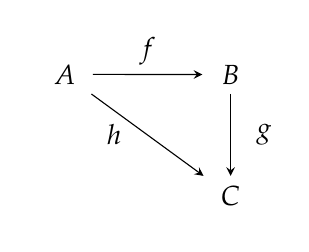
\begin{tikzpicture}
	\matrix (m) [matrix of math nodes,row sep=3em,column sep=4em,minimum width=2em]
	{
	A & B  \\ 
		& C\\};
	\path[-stealth]
		(m-1-1) edge node [above] {$f$} (m-1-2)
	(m-1-1) edge node [left]  {$h~~$} (m-2-2)
	(m-1-2) edge node [right] {$~~g$} (m-2-2);
\end{tikzpicture}
\\ 	
It will be said to \textit{commute} if $h = g\circ f$. The point is that the diagram offers 
two paths from $A$ to $C$, either by composing to follow $f$ and then $g$, or by 
following h directly. Commutativity means that the two paths amount to 
the same thing. A more complex diagram, like the previous one, is said to 
be commutative when all possible triangles that are parts of the diagram 
are themselves commutative. This means that any two paths of arrows in 
the diagram that start at the same object and end at the same object 
compose to give the same overall arrow. By a \textit{diagram} $D$ in a 
category $\mathscr C$ we simply mean a collection of $\mathscr C$-objects $d_j, d_k,...$ together 
with some $\mathscr C$-arrows $g: d_j \to d_k$ between certain of the objects in the 
diagram. (Possibly more than one arrow between a given pair of objects, 
possibly none). 
A \textit{cone} for diagram $D$ consists of a $\mathscr C$-object $c$ together with a $\mathscr C$-arrow 
$c\to d_j$ for each object $f_j$ in $D$, such that
		\newline
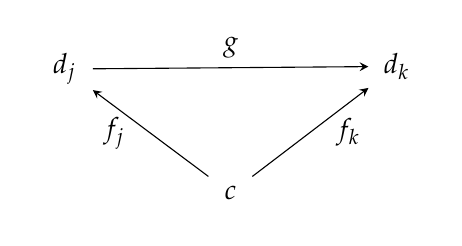
\begin{tikzpicture}
	\matrix (m) [matrix of math nodes,row sep=3em,column sep=4em,minimum width=2em]
	{
	d_j  & & d_k \\ 
		& c  & \\};
	\path[-stealth]
	(m-1-1) edge node [above] {$g$} (m-1-3)
	(m-2-2) edge node [left]  {$f_j~~$} (m-1-1)
	(m-2-2) edge node [right] {$~~f_k$} (m-1-3);
\end{tikzpicture}
\\ 	
 commutes, whenever g is an arrow in the diagram $D$. We use the 
symbolism $\left\{f_j: c\to d_j\right\}$ to denote a cone for $D$. 


A \textit{limit} for a diagram $D$ is a $D$-cone $\left\{f_j: c\to d_j\right\}$ with the property that for 
	any other $D$-cone $\left\{f'_j: c'\to d_j\right\}$ there is exactly one arrow $f:c' \to c$ such 
			\newline
	\begin{tikzpicture}
		\matrix (m) [matrix of math nodes,row sep=3em,column sep=4em,minimum width=2em]
		{
			  & d_j &  \\ 
		c'	&  & c \\};
		\path[-stealth]
		(m-2-1) edge node [above] {$g$} (m-2-3)
		(m-2-1) edge node [left]  {$f'_j~~$} (m-1-2)
		(m-2-3) edge node [right] {$~~f_j$} (m-1-2);
	\end{tikzpicture}
	\\ 	
		commutes for every object $d_j$ in $D$. 
		This limiting cone, when it exists, is said to have the \textit{universal property} 
		with respect to $D$ -cones.
		 A limit for 
		diagram $D$ is unique up to isomorphism.%:- if {ft: �> a\} and {f-:c'�> d;} 			are both limits for D, then the unique commuting arrow f: c'� above is 			iso (its inverse is the unique commuting arrow c-�*c' whose existence 			follows from the fact that {/,': c' �> dj is a limit). 
		% It is universal amongst such cones-any other 		D-cone factors uniquely through it as in the last diagram.		


\begin{definition}\label{pull_back_defn}\cite{goldblatt:topoi}
	A \textit{pullback} of a pair $a \xrightarrow{f}c \xleftarrow{g} b$ of $\mathscr C$-arrows with a common codomain 
	is a limit in $\mathscr C$ for the diagram 
			\newline
\begin{tikzpicture}
	\matrix (m) [matrix of math nodes,row sep=3em,column sep=4em,minimum width=2em]
	{
		& b  \\ 
		a	&  c \\};
	\path[-stealth]
	(m-1-2) edge node [right]  {$g$} (m-2-2)
	(m-2-1) edge node [above] {$f$} (m-2-2);
\end{tikzpicture}
\\ 	
	
\end{definition}
\subsection{Functors}
\begin{definition}\label{functor_defn}\cite{goldblatt:topoi}
A \textit{functor} $F$ from category $\mathscr{C}$ to category $\mathscr{D}$ is a function that assigns 
\begin{enumerate}
	\item [(i)]
 to each $\mathscr{C}$-object $a$, a $\mathscr{D}$-object $F(a)$; 
\item[(ii)] to each $\mathscr{C}$-arrow $f:a \to b$ a $\mathscr{D}$-arrow $F(f): F(a) \to F(b)$, 
such that 
\begin{enumerate}
	\item[(a)]  $F\left(\mathbb 1_a\right) = \mathbb 1_{F\left(a\right)}$ for all  $\mathscr{C}$-objects $a$, i.e. the identity arrow on $a$ is assigned 
	the identity on $F\left(a\right)$,
	\item[(b)]  $F\left(g\circ f\right)=F\left(g\right)\circ F\left( f\right) $, whenever $g \circ f$ is defined. 
	This last condition states that the $F$-image of a composite of two arrows 
	is the composite of their $F$-images.
\end{enumerate}


\end{enumerate}
 We write $F:\mathscr{C}\to \mathscr{D}$ or  $\mathscr{C}\xrightarrow{F} \mathscr{D}$ to indicate that $F$ is a 
functor from $
\mathscr{C}$ to $\mathscr{D}$. Briefly then a functor is a transformation that 
"preserves" dom's, cod's, identities and composites. 
\end{definition}
If $a$ and $b$ are  $\mathscr{C}$-objects then a functor $\mathscr{C}\xrightarrow{F} \mathscr{D}$ yields a map
\be\label{f_ab_funct_eqn}
F_{a,b}:\mathscr{C}\left(a, b \right)  \to \mathscr{D}\left( F\left(a\right), F\left(b\right)\right)  
\ee
(cf. Notation \ref{category_not}).
\begin{definition}\label{funct_full_faithfull_defn}\cite{bass}
A functor $\mathscr{C}\xrightarrow{F} \mathscr{D}$ is said to be \textit{faithful} (resp. \textit{full}) if the given by \eqref{f_ab_funct_eqn} map is injective (resp. surjective).
\end{definition}
\begin{defn}\label{functor_contravariant_defn}
A \textit{contravariant} functor is one that reverses direction by mapping domains 
to codomains and vice versa. 
Thus $\mathscr{C}\xrightarrow{F} \mathscr{D}$ is a contravariant functor if it assigns to $f: a\to b$ an 
arrow $F(f):F(b)\to F(a)$, so that $F\left(\mathbb{1}_a\right)= \mathbb{1}_{F(a)}$ as before, but now 
$$
F\left( g\circ f\right) = F\left( f\right)\circ  F\left( g\right). 
$$
\end{defn}
\subsection{Natural transformations}\label{natural_transformation_sec}
\paragraph{}
Here I follow to \cite{goldblatt:topoi}.
Given two categories $\mathscr C$ and $\mathscr D$ we are going to construct a category, 
denoted $\mathrm{Funct}\left(\mathscr C, \mathscr D\right)$, or $\mathscr D^{\mathscr C}$, whose objects are the functors from $\mathscr C$ to $\mathscr D$. 
We need a definition of arrow from one functor to another. Let 
$F: \mathscr C\to \mathscr D$ and $G: \mathscr C\to \mathscr D$ be two functors. For any $\mathscr C$-object $a$ we define a $\mathscr D$-arrow $\tau_a : F\left(a\right)\to  G\left(a\right)$. We require that each  $\mathscr C$-arrow $f: a \to b$  gives rise to a diagram 
	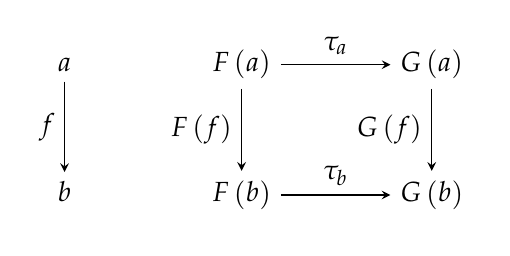
\begin{tikzpicture}
	\matrix (m) [matrix of math nodes,row sep=3em,column sep=4em,minimum width=2em]
	{
	a	& F\left(a \right)  &   G\left(a \right)\\ 
		b	& F\left(b \right)  &   G\left(b \right) \\};
	\path[-stealth]
	(m-1-1) edge node [left]  {$f$} (m-2-1)
	(m-1-2) edge node [above] {$\tau_a$} (m-1-3)
	(m-2-2) edge node [above]  {$\tau_b$} (m-2-3)
	(m-1-2) edge node [left]  {$F\left( f \right)$} (m-2-2)
	(m-1-3) edge node [left]  {$G\left( f \right)$} (m-2-3);
\end{tikzpicture}
\\ 	
that commutes.
%a F(a) Ta > G(a) Ftf)  F(b) T"  G(b) that commutes. Thus  and provide a categorical way of turning the F-picture of f:a-*b into its G-picture. 
In summary then, a \textit{natural transformation} from functor $F: \mathscr C\to \mathscr D$ and $G: \mathscr C\to \mathscr D$  to functor $F: \mathscr C\to \mathscr D$ and $G: \mathscr C\to \mathscr D$  is an assignment $\tau$ that provides, for each $\mathscr C$-object $\mathscr D$-arrow $\tau_a :F(a) \to G(a)$, such that for any $\mathscr C$-arrow $f:a\to b$, the above diagram commutes in $\mathscr D$, i.e. $\tau_b \circ F(f)= G(f)\circ \tau_a$. We use the symbolism $\tau: F\to G$, or $F \xrightarrow{\tau}G$, to denote that $\tau$ is a natural transformation from $F$ to $G$. The arrows $\tau_a$ are called the \textit{components} of $a$. Now if each component $\tau_a$ of $a$ is an iso arrow in $\mathscr D$ then  case we call $\tau$ a \textit{natural isomorphism}. Each $\tau_a: F(a)\to G(a)$ then has an inverse $\tau_a^{-1}: G(a) \to F(a)$, and these $\tau^{-1}_a$'s form the components of a natural isomorphism $\tau^{-1}: G \to F$. We denote natural isomorphism by $\tau: F \cong G$. 
\begin{example}
The identity natural transformation $\mathbb{1}_F :F\to F$ assigns to each object $a$, the identity arrow $\mathbb{1}_{F(a)}:F(a)\to F(a)$. This is clearly a natural isomorphism. 
\end{example}

	\begin{definition}\label{category_equivalence_definition}\cite{goldblatt:topoi}
	A functor $F: \mathscr C\to  \mathscr D$ is called an \textit{equivalence of categories} if there 
	is a functor $G: \mathscr D\to  \mathscr C$ such that there are natural isomorphisms $\tau : 1_{\mathscr C} \cong G \circ F$, and $\sigma : 1_{\mathscr D} \cong F \circ G$, from the identity functor on ${\mathscr C}$ to $ G \circ F$, and 
	from the identity functor on ${\mathscr D}$ to $ F \circ G$.
	
	Categories $\mathscr C$ and $\mathscr D$ are \textit{equivalent},  $\mathscr C$ and $\mathscr D$ when there exists an equivalence $F: \mathscr C\to  \mathscr D$ .
\end{definition}

	\section{Grothendieck topology and sheaves}

\subsection{Sites}\label{appendix_etale_sec}
\begin{definition}\label{pullback_defn}\cite{milne:lec}
For $X$ an object of a category $\mathscr C$, $\mathscr C/X$ denotes the category whose objects are the morphisms $U\to X$ in $\mathscr C$
and whose arrows are the commutative diagrams 
			\newline
\begin{tikzpicture}
	\matrix (m) [matrix of math nodes,row sep=3em,column sep=4em,minimum width=2em]
	{
		U  &  & U'\\ 
	 & X &\\};
	\path[-stealth]
	(m-1-1) edge node [above] {} (m-1-3)
	(m-1-1) edge node [above]  {} (m-2-2)
	(m-1-3) edge node [right]  {} (m-2-2);
\end{tikzpicture}
\\
A morphism $U \to U'$ making this diagram commute is also referred to as an $X$-morphism. The \textit{fibre product}  $U_1\times_X U_2$ of morphisms $\varphi_1: U_1\to X$,  $\varphi_2: U_2\to X$ in $\mathscr C$ is their product in the category $\mathscr C$. Thus, there is a commutative diagram 
			\newline
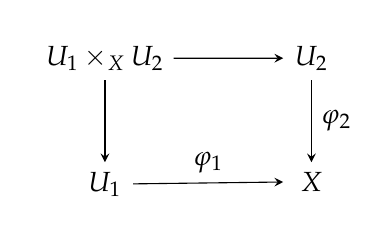
\begin{tikzpicture}
	\matrix (m) [matrix of math nodes,row sep=3em,column sep=4em,minimum width=2em]
	{
		U_1\times_X U_2 & U_2\\ 
		U_1 & X\\};
	\path[-stealth]
	(m-1-1) edge node [above] {} (m-1-2)
	(m-2-1) edge node [above]  {$\varphi_1$} (m-2-2)
	(m-1-1) edge node [right]  {} (m-2-1)
	(m-1-2) edge node [right] {$\varphi_2$} (m-2-2);
\end{tikzpicture}
\\
having the obvious universal property. 

\end{definition}
\begin{definition}\label{site_defn}\cite{milne:lec}
A category $\mathscr C$  
together with, for each object $U$ of $\mathscr C$, a distinguished set of families of maps $\left\{U_\iota \to U\right\}_{\iota\in I}$, called the \textit{coverings} of $U$, 
satisfying the following axioms: 
\begin{enumerate}
	\item[(a)] for any covering $\left\{U_\iota \to U\right\}_{\iota\in I}$ and any morphism $U \to V$ in $\mathscr C$, the fibre products 
		$U_\iota\times_U V$ exist, and $\left\{U_\iota\times_U V \to V\right\}_{\iota\in I}$ is a covering of $V$; 
	\item[(b)] if $\left\{U_\iota \to U \right\}_{\iota\in I}$ is a covering of $U$, and if for each $\iota \in I$, $\left\{V_{\iota j}\times_U V \to U_\iota  \right\}_{j \in I_\iota}$	is a 
	covering of $U_\iota$, then the family $\left\{V_{\iota j }\to U\right\}_{\iota j}$ is a covering of $U$; 
	\item[(c)] for any $U$ in $\mathscr C$, the family $\left\{U\xrightarrow{\Id}U \right\}$ consisting of a single map is a covering of $U$. 
\end{enumerate}
The system of coverings is then called a \textit{(Grothendieck) topology}, and $\mathscr C$  together with 
the topology is called a \textit{site}. If $\mathbf T$  
is a site, then $\mathrm{Cat}\left( \mathbf T\right)$  denotes the underlying category. 

\end{definition}

\begin{definition}\label{etale_presheaf_defn}\cite{milne:lec}
A \textit{presheaf of sets} on a site $\mathbf T$ 
is a contravariant functor $\sF$ from $\mathrm{Cat}\left( \mathbf T\right)$ to the category of sets. Thus,  $\sF\left(U \right) $
to each object $F$ in $\mathrm{Cat}\left( \mathbf T\right)$ 
attaches a set $\sF\left(U \right)$ , and to each morphism $\phi: U \to V$
in $\mathrm{Cat}\left( \mathbf T\right)$, a map $\sF\left(\varphi\right):\sF\left(V \right)\to \sF\left(U \right)$. Note that the notion of a presheaf on T 
does not depend on the 
coverings. We sometimes denote $\sF\left(\varphi\right)$ by $a \mapsto a|_U$.

\end{definition}
Similarly, a presheaf of (Abelian) groups or rings on $\mathbf T$ is a contravariant functor from
$\mathrm{Cat}\left( \mathbf T\right)$ to the category of (Abelian) groups or rings.
\begin{definition}\label{etale_sheaf_defn}\cite{milne:lec}
A \textit{sheaf} on $\mathbf T$ 
is a presheaf $\sF$ 
that satisfies the sheaf condition: 
\be\label{etale_sheaf_eqn}
\sF \left(U\right) \to \prod_{\iota \in I} \sF \left(U_\iota \right)\rightrightarrows  \prod_{\iota, j \in I\times I} \sF \left(U_\iota \times_U U_j\right)
\ee
is exact for every covering $\left\{U_\iota \to U\right\}$ Thus $\sF$ 
is a sheaf if the map 
$$
f \mapsto \left\{f_{U_\iota }\right\}:\sF \left(\sU\right) \to \prod_{\iota \in I} \sF \left(U_\iota \right)
$$
identifies $\sF\left( U\right)$ with the subset of the product consisting of families $\left\{f_\iota\right\}$such that 
$$
f_\iota|_{U_\iota \times_U U_j}= f_j|_{U_\iota \times_U U_j}
$$
for all $\iota, j \in I$ 
When $\mathbf T$ 
is the site arising from a topological space, these definitions coincide with the 
usual definitions. 
	
\end{definition}

There are categories $\mathbf{PreSh}\left(\mathbf T \right)\to \mathbf{Sh}\left(\mathbf T\right)$ of presheaves an sheave. Moreover there is a forgetful functor  functor $\mathfrak{Forget} : \mathbf{Sh}\left(\mathbf T \right)\to \mathbf{PreSh}\left(\mathbf T \right)$.

\begin{statement}\label{site_sheaf_stmt}\cite{johnstone:topos}
	There is an adjoint $\mathfrak{Ass} : \mathbf{PreSh}\left(\mathbf T  \right)\to \mathbf{Sh}\left(\mathbf T \right)$ to the given by the forgetful functor $\mathfrak{Forget} : \mathbf{Sh}\left(\mathbf T  \right)\to \mathbf{PreSh}\left(\mathbf T \right)$.
\end{statement}	
\begin{defn}\label{site_sheaf_ass_defn}\cite{johnstone:topos}
	The given by the Statement  \ref{site_sheaf_stmt} functor $\mathfrak{Ass} : \mathbf{PreSh}\left(\mathbf T  \right)\to \mathbf{Sh}\left(\mathbf T \right)$  is said to be an  \textit{associated sheaf functor}.
\end{defn}	
\begin{statement}\cite{johnstone:topos}
If $\mathbf T$ is a site then a category $\mathbf {Ab} \left(\mathbf T \right)$ of sheaves of Abelian groups has
enough injective objects.
\end{statement}

\subsection{Cohomology. Definition and basic properties}
\paragraph{}
Here I follow to \cite{milne:lec}. The functor
\bean
\Ga\left(X, \cdot \right) : \mathbf {Ab} \left(\mathbf T \right) \to \mathbf {Ab} ,\\
\mathscr F \mapsto \mathscr F\left(X \right) 
\eean
of global sections is left exact, and we define $H^r\left(X,~ \cdot ~\right)$ to be its $r^{\text{th}}$ right derived functor. Explicitly, for a sheaf $\mathscr F$, choose an injective resolution
$$
0 \to \mathscr F \to \mathscr I^0\to \mathscr I^1\to \mathscr I^2 \to ...
$$
and apply the functor $\Ga\left(X, \cdot \right)$ to obtain a complex
$$
\Ga\left(X,\ \mathscr I^0  \right) \to \Ga\left(X, \mathscr I^1  \right) \to \Ga\left(X, \mathscr I^2  \right) \to ... 
$$
This is no longer exact (in general), and $H^r\left(X,\ \mathscr I^0  \right)$ is defined to be its $r^{\text{th}}$ cohomology
group. The theory of derived functors shows:
\begin{enumerate}
	\item [(a)] $H^0\left(X,\ \mathscr F  \right)\Ga\left(X,\ \mathscr F \right)$ for any sheaf $\mathscr F$;
	\item [(b)] if $\mathscr I$ is injective, then $H^r (X,\mathscr I )= 0$ for $r > 0$;
	\item [(c)]  short exact sequence of sheaves
$0\to \mathscr F' \to \mathscr F \to \mathscr F'' \to 0$	gives rise to a long exact sequence
$$
0 \to H^0\left(X, \mathscr F'  \right) \to\left(X, \mathscr F  \right) \to H^0\left(X, \mathscr F''  \right) \to H^1\left(X,\ \mathscr F'  \right) \to ...
$$
and the association of the long exact sequence with the short exact sequence is functional.
\end{enumerate}
Moreover, the functors $H^r\left( X,~ \cdot ~\right)$  are uniquely determined (up to a unique isomorphism)
by the properties (a), (b) and (c).

\subsection{\v{C}ech cohomology}
\paragraph{} Here I follow to \cite{milne:lec}. Let $\mathscr U \bydef \left\{U_\iota \to X\right\}_{\iota \in I}$ be  covering of $X$, and let $\mathscr P$ be a presheaf of Abelian groups. Define
$$
C^r\left( \mathscr U, \mathscr P\right)\bydef \prod_{\left(\iota_0,.... \iota_r\right) \in I^{r+1}} \mathscr P\left(U_{\iota_0,.... \iota_r} \right)\quad \text{where} \quad U_{\iota_0,.... \iota_r} \bydef U_{\iota_0}\times_X...\times_XU_{\iota_r}. 
$$
For $s \in C^r\left( \mathscr U, \mathscr P\right)$ define $d^rs \in C^{r+1}\left( \mathscr U, \mathscr P\right)$ by the rule
$$
d^rs_{\iota_0,..., \iota_{r + 1}}\bydef \sum_{j = 0}^{r + 1}\left(-1 \right) \mathrm{res}_j\left(s_{\iota_0,..., \iota_{j-1},...,\iota_{j+1},..., \iota_{r + 1}} \right)  
$$
where $\mathrm{res}_j$ is the restriction map corresponding to the projection map
$$
U_{\iota_0,..., \iota_{r + 1}}\mapsto U_{\iota_0,..., \iota_{j-1},...,\iota_{j+1},.., \iota_{r + 1}}
$$
As in the classical case, one verifies by a straightforward calculation that
$$
C^\bullet\left( \mathscr U, \mathscr P\right) \bydef C^0\left( \mathscr U, \mathscr P\right) \to C^r\left( \mathscr U, \mathscr P\right) \xrightarrow{d_r} C^r\left( \mathscr U, \mathscr P\right)\to ...
$$
is a complex. Define
$$
\check{H}^r\left( \mathscr U, \mathscr P\right) \bydef H^r\left(C^\bullet\left( \mathscr U, \mathscr P\right)   \right). 
$$
It is called the $r^{\text{th}}$ \textit{\v{C}ech cohomology group} of $\mathscr P$ relative to the covering $\mathscr U$.
Note that
$$
\check{H}^r\left( \mathscr U, \mathscr P\right)= \ker\left(\prod \mathscr P_\iota \rightrightarrows \prod \mathscr P_{\iota,j} \right) 
$$
Therefore, for a sheaf $\mathscr F$ one has
$$
\check{H}^0\left( \mathscr U, \mathscr F\right)=\Ga\left( \mathscr U, \mathscr F\right).
$$
A second covering $\mathscr V \bydef \left\{V_j\to X \right\}_{j \in J}$ of $X$ is called a \textit{refinement} of $\mathscr U$ if there is a
map $\tau : J\to I$ such that $V_j \to X$ factors through $U_{\tau_j}\to X$ for all $j \in J$ . The choice of
a $\tau$ and $X$-morphisms $\varphi_{j}: V_j \to U_{\tau_j}$ for each $j$ determines a map of complexes
\bean
\tau^\bullet: C^\bullet\left( \mathscr U, \mathscr P\right)\to C^\bullet\left( \mathscr V, \mathscr P\right),\\
\left( \tau^r s_{j_0,..., j_{r}} \right) \bydef s_{\tau j_0,..., \tau j_{r}}.
\eean
As in the classical case, one verifies that the map on cohomology groups
$$
\rho \left(\mathscr U, \mathscr V \right): \check{H}^r\left( \mathscr U, \mathscr P\right)\to \check{H}^r \left( \mathscr V, \mathscr P\right)
$$
is independent of all choices. We may pass to the limit over all coverings, and so obtain limits
\be\label{chech_eqn}
\check{H}^r\left(X, \mathscr P\right)\bydef \varinjlim_{\mathscr U}\check{H}^r\left( \mathscr U, \mathscr P\right).
\ee
\begin{defn}\label{chech_defn}
The  \textit{\v{C}ech cohomology groups} are given by equation \eqref{chech_eqn}
\end{defn}
These groups  have the following properties:
\begin{enumerate}
	\item [(a)] $\check{H}^0\left(X, \mathscr F\right)= \Ga\left( X, \mathscr F\right)$ for any sheaf $\mathscr F$ on $X$;
	\item[(b)] $\check{H}^0\left(X, \mathscr I\right)$, $r > 0$, for all injective sheaves $\mathscr I$.
\end{enumerate}
\begin{empt}
	For any Abelian group $A$ one can define a constant presheaf $\mathscr P$ of Abelian groups. This presheaf sets $A$ for any object of $\mathrm{Cat}\left( \mathbf T\right)$ and an identical morphism $A\xrightarrow{\Id_A}A$ for any morphism of $\mathrm{Cat}\left( \mathbf T\right)$. 
	 We use a following notation
	\be\label{etale_hom_a_eqn}
	\check{H}^r\left(X,  A\right)\bydef \check{H}^r\left(X, \mathscr P\right).
	\ee
\end{empt}

 	
 \end{appendices}
 

 
\section*{Acknowledgment}


\paragraph*{}
I am very grateful to Prof. Joseph C Varilly  and Arup Kumar Pal
 for advising me on the properties of Moyal planes and equivariant spectral triples respectively. Author would like to acknowledge members of the Moscow State University Seminars
 "Noncommutative geometry and topology", "Algebras in analysis" leaded by professors A. S. Mishchenko and  A. Ya. Helemskii for a discussion
 of this work. I am grateful to my grandfather Petr who forested my mind and my grandson Petr who  watched my work during the quarantine.
 
  
  
  
 

 
 \begin{thebibliography}{10}
 	
%\bibitem{lie_groupoids_coov}  CORRECT TURKISH

%I. I�en, M. G�rsoy, A. �zcan \textit{Coverings of Lie groupoids} 	Turk J Math, 35 (2011) , 207 � 218. 	c�T  UB ITAK, doi:10.3906/mat-0902-2, 2011.
 	
 	\bibitem{alekseev_bytsko:wilson_nc_tori} Anton Alekseev, Andrei Bytsko, {\it 	Wilson lines on noncommutative tori}. arXiv:hep-th/0002101, 2000.
 	
 	\bibitem{apt_mult}	Charles A. Akemann, Gert K. Pedersen, Jun Tomiyama. \textit{Multipliers of $C^*$-algebras}. Journal of Functional Analysis Volume 13, Issue 3, July 1973, Pages 277-301, 1973.
  
 	
 	\bibitem{Ambjorn:2000cs}  J.~Ambjorn, Y.~M.~Makeenko, J.~Nishimura and R.~J.~Szabo,  {\it Lattice gauge fields and discrete noncommutative Yang-Mills theory}.  JHEP {\bf 0005}, 023 hep-th/0004147, 2000.
 	
 	
 	%\bibitem{akhi:fa}	N. I. Akhiezer, I. M. Glazman. \textit{Theory of Linear Operators in Hilbert Space}. Dover Publications, New York, 1961, 1963.
 	
 	\bibitem{antoine:part_o} Antoine, Jean-Pierre, Inoue, Atsushi, Trapani, C.  \textit{Partial *- Algebras and Their Operator Realizations}. SPRINGER-SCIENCE+BUSINESS MEDIA, B.V. 2002.
 	
 	
 	\bibitem{antoine:part_s} J.-P. Antoine, F. Mathot, \textit{Partial *-algebras of closed operators and their commutants. I. General
 		structure}. Ann. Inst. H. Poincar� 46, 299�324 (1987), 1987.
 	
 	\bibitem{arveson:c_alg_invt} W. Arveson. {\it An Invitation to $C^*$-Algebras}, Springer-Verlag. ISBN 0-387-90176-0, 1981.
 	
 	
 	\bibitem{atiyah_b_s}
 	M. F. Atiyah, R. Bott and A. Shapiro, \textit{Clifford Modules}, Topology {\bf 3} (1964), 3--38.  1964.
 	
 	%\bibitem{ant_azz_scan:flat_k}Paolo Antonini, Sara Azzali, Georges Skandalis {\it Flat bundles, von Neumann algebras and $K$-theory with $\mathbb{M}hbb{R}/\mathbb{M}hbb{Z}$-coefficients}, arXiv:1308.0218, 2013.
 	
 	\bibitem{auslander:galois} M. Auslander; I. Reiten; S.O. Smal\o{}. \textit{Galois actions on rings and finite Galois coverings}. Mathematica Scandinavica (1989), Volume: 65, Issue: 1, page 5-32, ISSN: 0025-5521; 1903-1807/e , 1989.
 	
 		\bibitem{bfss} T. Banks, W. Fischler, S.H. Shenker and L. Susskind, Phys.
 	Rev. {\bf
 		D55} (1997) 5112 [{\tt hep-th/9610043}].
 	
 	\bibitem{bss} T. Banks, N. Seiberg and S.H. Shenker, Nucl. Phys. {\bf B490}
 	(1997) 91
 	[{\tt hep-th/9612157}].
 	
 	
 

%\bibitem{bezandry_diagana:bound_unbound}Paul H. Bezandry, Toka Diagana {\it Bounded and Unbounded Linear Operators}, in {\it Almost Periodic Stochastic Processes}, Springer, 2011.

%\bibitem{ballentine:qm} Leslie E Ballentine. {\it Quantum Mechanics: A Modern Development.} World Scientific Publishing Co. Pte. Ltd. 2000.
\bibitem{bass} H. Bass. {\it Algebraic K-theory.} W.A. Benjamin, Inc. 1968. 


\bibitem{becker:sting_m}Katrin Becker, Melanie Becker, John H. Schwarz. \textit{String Theory and M-Theory: A Modern Introduction}. Cambridge University Press. 2007.

\bibitem{blackadar:ko} B. Blackadar. {\it K-theory for Operator Algebras}, Second edition. Cambridge University Press. 1998.

\bibitem{blackadar:oa} B. Blackadar. \textit{Operator Algebras: Theory of C*-Algebras and von Neumann Algebras}, (Encyclopaedia of Mathematical Sciences), Springer,  2006.

\bibitem{blackadar:shape_theory} B. Blackadar, {\it Shape theory for $C^*$-algebras}, Math. Scand. 56 , 249-275, 1985.

\bibitem{blecher_merdy} David P. Blecher, Christian Le Merdy. \textit{Operator algebras and their modules - an operator space approach}, CLARENDON PRESS - OXFORD, 2004.

%\bibitem{blecher:hilb_gen} D.P. Blecher. {\it A generalization of Hilbert modules}, J.Funct. An. 136, 365-421 1996.

\bibitem{bogachev_measure_v1}V. I. Bogachev. {\it Measure Theory} (volume 1). Springer-Verlag, Berlin, 2007.

\bibitem{bogachev_measure_v2}V. I. Bogachev. {\it Measure Theory}. (volume 2). Springer-Verlag, Berlin, 2007.

\bibitem{bogopolsky:group_theory}Oleg Bogopolski. \textit{Introduction to Group Theory}. European Mathematical Society. 2008.


\bibitem{bourbaki_sp:gt} N. Bourbaki, {\it Elements of Mathematics. General Topology}, Part 1. \newline HERMANN, \'{E}DITEURS DES SCIENCES ET DAS ARTS \newline 115 Boulevard Saint-Germain. Paris \newline ADDISON-WESLEY PUBLISHING COMPANY. \newline Reading, Massachusets - Palo Ito - London - Don Mills, Ontario \newline A translation of \newline \'{E}L\'{E}MENTS DE MATH\'{E}MATIQUE, TOPOLOGIE G\'{E}N\'{E}RALE, \newline originally published in French by Hermann, Paris. 1966.

\bibitem{bredon:sheaf} Bredon, Glen E. (1997), \textit{Sheaf theory}. Graduate Texts in Mathematics, 170 (2nd ed.), Berlin, New York: Springer-Verlag.  ISBN 978-0-387-94905-5, MR 1481706 (oriented towards conventional topological applications), 1997.


\bibitem{brickell_clark:diff_m} F. Brickell and R. S. Clark.
{\it Differentiable manifolds; An introduction.} London; New York: V. N. Reinhold Co., 1970.





\bibitem{brown:proper_groupoids}Jonathan Henry Brown. \textit{Proper actions of groupoids on $C^*$-algebras}. arXiv:0907.5570, 2009.

\bibitem{brown:stable} Lawrence G. Brown, Philip Green, and Marc A. Rieffel. \textit{Stable isomorphism and strong Morita equivalence of $C^*$-algebras}. Pacific J. Math., Volume 71, Number 2 (1977), 349-363. 1977.

\bibitem{BroGreRie}L.~G. Brown, P.~Green, and M.~A. Rieffel.  \textit{Stable isomorphism and strong {Morita} equivalence of	{$C^*$}-algebras}.\newblock { Pacific J. Math.} {\bf 71} (1977), 349--363. 1977.

\bibitem{brzezinsky:flat_co}Tomasz Brzezinski \textit{Flat connections and (co)modules}, arXiv:math/0608170, 2006.
\bibitem{candel:foliI}Alberto Candel, Lawrence Conlon. \textit{Foliations I}. Graduate Studies in Mathematics, American Mathematical Society (1999), 1999.
%
\bibitem{candel:foliII}Alberto Candel, Lawrence Conlon. \textit{Foliations II}. American Mathematical Society; 1 edition (April 1 2003), 2003.

\bibitem{chun-yen:separability} Chun-Yen Chou. {\it Notes on the Separability of $C^*$-Algebras.} TAIWANESE JOURNAL OF MATHEMATICS Vol. 16, No. 2, pp. 555-559, April 2012 This paper is available online at http://journal.taiwanmathsoc.org.tw , 2012.

\bibitem{mont:hopf-morita} M. Cohen, D. Fischman, S. Montgomery. \textit{Hopf Galois extensions, smash products, and Morita equivalence}. Journal of Algebra Volume 133, Issue 2, September 1990, Pages 351-372, 1990.

\bibitem{clarisson:phd} Clarisson Rizzie Canlubo. \textit{Non-commutative Covering Spaces and Their Symmetries}. PhD thesis. University of Copenhagen. 2017.

\bibitem{connes:foli_survey} A. Connes. \textit{A survey of foliations and operator algebras}. Operator algebras and applications, Part 1, pp. 521-628, Proc. Sympos. Pure Math., 38, Amer. Math. Soc, Providence, R.I., 1982; MR 84m:58140. 1982.

	\bibitem{cds} A. Connes, M.R. Douglas and A. Schwarz, J. High Energy Phys.
{\bf 9802}
(1998) 003 [{\tt hep-th/9711162}].


\bibitem{connes:ncg94} Alain Connes. {\it Noncommutative Geometry}, Academic Press, San Diego, CA,  661 p., ISBN 0-12-185860-X, 1994.

\bibitem{connes:c_alg_dg} Alain Connes. {\it $C^*$-algebras and differential geometry}. arXiv:hep-th/0101093, 2001.



\bibitem{connes_landi:isospectral} Alain Connes, Giovanni Landi. {\it Noncommutative Manifolds the Instanton Algebra and Isospectral Deformations}, arXiv:math/0011194, 2001.

\bibitem{connes_lott:particle} Connes, Alain, Lott, John. \textit{Particle models and noncommutative geometry.} Nuclear Physics B - Proceedings Supplements (1991/01) 18(2): 29-47, 1991

\bibitem{connes_rieffel:nc_ym}A. Connes, Marc A. Rieffel \textit{Yang-Mills for noncommutative two-tori}. 1987 30 pages Published in: Contemp.Math. 62 (1987) 237-266, In *Li, M. (ed.) et al.: Physics in non-commutative world, vol. 1* 46-62. 1987.

\bibitem{cra_moe:nhaus} M. Crainic and I. Moerdijk. \textit{A remark on sheaf  theory for non-Hausdorff manifolds}. Tech. Report 1119, Utrecht University, 1999.

\bibitem{cuntz:k_c_a}  J. Cuntz. \textit{$K$-theory for certain $C^*$-algebras}, Ann. of Math. (2) 113:1, 1981.

%\bibitem{vandaele:dqg} A. Van Daele. \textit{Discrete Quantum Groups.} Academic Press, San Diego, CA,  661 p., ISBN 0-12-185860-X, 1994. Journal of Algebra Volume 180, Issue 2, March 1996, Pages 431-444, 1996.


\bibitem{dabrowski:product}
Ludwik D\k{a}browski, Giacomo Dossena. \textit{Product of real spectral triples}. International Journal of Geometric Methods in Modern Physics, Volume 08, Issue 08, December 2011.
\bibitem{dix:profinite} John D. Dixon, Edward W. Formanek, John C. Poland, Luis Ribes. \textit{Profinite completion and isomorphic finite quotients}. Journal of Pure and Applied Algebra 23 (1982) 227-23 1, 1982.

\bibitem{Driver} B.~Driver {\it Classifications of bundle connection pairs by parallel translation and lassos}.
J.\ Funct.\ Anal.\ {\bf 83}, no.\ 1, (1989).
\bibitem{engelking:general_topology} Ryszard Engelking. \textit{General topology}, PWN, Warsaw. 1977.

\bibitem{varilly_bondia:phobos}Jos\'e M.  Gracia-Bond\'{\i}a, Joseph C.  V\'arilly.  \textit{Algebras of Distributions suitable for phase-space quantum mechanics. I}. Escuela de Matem\'{a}tica, Universidad de Costa Rica, San Jos\'e, Costa Rica J. Math. Phys 29 (1988), 869-879, 1988.

\bibitem{varilly_bondia:deimos}
J. C. V\'arilly and J. M. Gracia-Bond\'{\i}a, \textit{Algebras of distributions suitable for phase-space quantum mechanics II: Topologies on the Moyal algebra}, J. Math. Phys. {\bf 29} (1988), 880--887. 1988.
	
%\bibitem{hajac:s_conn}	P. M. Hajac, \textit{Strong connections on quantum principal bundles},Commun. Math. Phys. {\bf 182} (1996), 579--617. 1996.	

%\bibitem{bruckler:tensor} Franka Miriam Br\"uckler. {\it Tensor products of $C^*$-algebras, operator spaces and Hilbert $C^*$-modules}. Mathematical Communications 4(1999), 1999.

\bibitem{do_carmo:rg} Manfredo P. do Carmo. {\it Riemannian Geometry.} Birkh\"auser, 1992.

 
\bibitem{chakraborty_pal:quantum_su_2} Partha Sarathi Chakraborty,  Arupkumar Pal. \textit{Equivariant spectral triples on the quantum $SU(2)$ group}. arXiv:math/0201004v3, 2002.

\bibitem{chakraborty_pal:inv_hom} Partha Sarathi Chakraborty,  Arupkumar Pal. \textit{An invariant for homogeneous spaces of compact quantum groups}. Advances in Mathematics. 301 (2016) 258� 2016.

%\bibitem{chang:fermionic} Ee Chang-Young, Hiroaki Nakajima, Hyeonjoon Shin. {\it Fermionic $T$-duality and Morita Equivalence}, arXiv:1101.0473, 2011.

%\bibitem{morita_hopf_galois}S. Caenepeel, S. Crivei, A. Marcus, M. Takeuchi. {\it Morita equivalences induced by bimodules over Hopf-Galois extensions.}arXiv:math/0608572, 2007.



%\bibitem{cheng_li:gauge}Cheng, T.-P.; Li, L.-F. {\it Gauge Theory of Elementary Particle Physics}. Oxford University Press. ISBN 0-19-851961-3. 1983.

%\bibitem{connes:gravity}A. Connes. {\it Gravity coupled with matter and foundation of noncommutative geometry�\}, Commun. Math. Phys. 182 (1996), 155�176. 1996.

%\bibitem{connes:c_alg_dg} Alain Connes. {\it $C^*$-algebras and differential geometry}. arXiv:hep-th/0101093, 2001.



%\bibitem{connes_marcolli:motives}
%Alain Connes, Matilde Marcolli. {\it Noncommutative Geometry, Quantum Fields and Motives},  American Mathematical Society, Colloquium Publications, 2008.

% \bibitem{connes_moscovici:local_index} A. Connes and H. Moscovici, {\it The local index theorem in noncommutative geometry"}. Geom. and Funct. Anal., 1996.


%\bibitem{cuntz_quillen:alg_ext} Joachim Cuntz, Daniel Quillen.  {\it Algebra extensions and nonsingularity}, J. Amer. Math. Soc. 8 251-289, 1995

%\bibitem{davis_kirk_at}James F. Davis. Paul Kirk. {\it Lecture Notes in Algebraic Topology}. Department of Mathematics, Indiana University, Blooming- ton, IN 47405, 2001.

\bibitem{dijkhuizen:so_doublecov} Dijkhuizen, Mathijs S. \textit{The double covering of the quantum group $SO_q(3)$}. Rend. Circ. Mat. Palermo (2) Suppl. (1994), 47-57. MR1344000, Zbl 0833.17019. 1994.

\bibitem{dixmier_a_r} Jacques Dixmier {\it Les C*-alg\`{e}bres et leurs repr\'esentations} 2e \'ed. Gauthier-Villars in Paris 1969.



\bibitem{dixmier_ca}Jacques Dixmier. \textit{$C^*$-Algebras}. University of Paris VI, North-Holland Publishing Company, 1977.

\bibitem{dixmier_tr}J. Dixmier. {\it Traces sur les $C^*$-algebras}. Ann. Inst. Fourier, 13, 1(1963), 219-262, 1963.

\bibitem{dosi:multi} Anar Dosi. \textit{Local operator spaces, unbounded operators and multinormed $C^*$-algebras}.      Journal of Functional Analysis 255(7):1724-1760. October 2008.


\bibitem{effros:loc_conv} E.G. Effros, C. Webster \textit{ Operator analogues of locally convex spaces}, in: Operator Algebras and Applications,Samos 1996, in: NATO Adv. Sci. Inst. Ser. C Math. Phys. Sci., vol. 495, Kluwer, Amsterdam, 1997.

\bibitem{elliot:an} Elliott H. Lieb, Michael Loss. \textit{Analysis}, American Mathematical Soc., 2001.


\bibitem{fell:operator_fields}J. M. G. Fell. \textit{The structure of algebras of operator fields}. Acta Math. Volume 106, Number 3-4 (1961), 233-280. 1961.

\bibitem{quasi_star_many} M. Fragoulopoulou, C. Trapani S. Triolo \textit{Locally convex quasi *-algebras with sufficiently many *-representations}.  J. Math. Anal. Appl. 388 (2012) 1180�1193, 2012.

\bibitem{quasi_star} Maria Fragoulopoulo, Camillo Trapani \textit{Locally Convex	Quasi *-Algebras 	and their	Representations}. Springer Nature Switzerland AG, 2020.


\bibitem{moyal_spectral} V. Gayral, J. M. Gracia-Bond\'{i}a, B. Iochum, T. Sch\"{u}cker, J. C. Varilly. {\it Moyal Planes are Spectral Triples}. arXiv:hep-th/0307241, 2003.

\bibitem{godement:sheaf} Roger Godement, \textit{Topologie Alg�brique et Th�orie des Faisceaux}. Actualit�s Sci. Ind. No. 1252. Publ. Math. Univ. Strasbourg. No. 13 Hermann, Paris. 1958.

\bibitem{cinfty_manifolds} Juan A. Navarro Gonz�lez, Juan B. Sancho de Salas. $\Coo$-\textit{Differentiable Spaces}. Springer.  2003.



%\bibitem{gilkey:odd_space}P.B. Gilkey. {\it The eta invariant and the $K$-theory of odd dimensional spherical space forms}.Inventiones mathematicae, Springer-Verlag, 1984.


%\bibitem{nicolas_ginoux:dirac_spectrum}Nicolas Ginoux. {\it The Dirac Spectrum.}Springer, Jun 11, 2009.

\bibitem{goldblatt:topoi} Robert Goldblatt. \textit{Topoi: The Categorial Analysis of Logic}. Revised edition of XLVII 445. Studies in logic and the foundations of mathematics, vol. 98. North-Holland, Amsterdam, New York, and Oxford, 1984, xvi + 551 pp. 1984.

\bibitem{varilly_bondia} Jos\'e M. Gracia-Bondia, Joseph C. Varilly, Hector Figueroa, {\it Elements of Noncommutative Geometry}, Springer, 2001.

\bibitem{green_schwarz_witten:superstring} {\it Superstring Theory: Volume 2, Loop Amplitudes, Anomalies and Phenomenology}. (Cambridge Monographs on Mathematical Physics)by Michael B. Green, John H. Schwarz, Edward Witten. 1988.


%\bibitem{gross_gauge}David J. Gross. {\it Gauge Theory-Past, Present, and Future} Joseph Henry Luborutoties, Ainceton University, Princeton, NJ 08544, USA. (Received November 3,1992).

%\bibitem{ful:gr_repr} Fulton William, Harris Joe. {\it Representation theory. A first course} Graduate Texts in Mathematics, Readings in Mathematics 129, New York: Springer-Verlag. 1991.
\bibitem{hartshorne:ag} Robin Hartshorne. {\it Algebraic Geometry.} Graduate Texts in Mathematics, Volume 52, 1977.



%\bibitem{halmos:set} Paul R.  Halmos {\it Naive Set Theory.} D. Van Nostrand Company, Inc., Prineston, N.J., 1960.


%\bibitem{helemsky:qfa} A. Ya. Helemsky. {\it Quantum Functional Analysis. Non-Coordinate Approach.} Providence, R.I. : American Mathematical Society, 2010.


\bibitem{hajac:toknotes}
{\it Lecture notes on noncommutative geometry and quantum groups}, Edited by Piotr M. Hajac.

\bibitem{hamermesh:group} M. Hamermesh. \textit{Group Theory and its Applications to Physical Problems}, Addison-Wesley, 1962.


\bibitem{harzheim:os} Egbert Harzheim. \textit{Ordered sets}.
Springer Science+Business Media, Inc. 2005.




%\bibitem{isaacs:auto} I.M. Isaacs. \textit{Automorphisms of matrix algebras over commutative rings}. Linear Algebra and its Applications, Volume 31, June 1980, Pages 215-231, 1980.

\bibitem{hilsum_scandalis:stab}Hilsum, Michel; Skandalis, Georges. \textit{Stabilit� des $C^*$-alg�bres de feuilletages}. Annales de l'Institut Fourier, Volume 33 (1983) no. 3, p. 201-208, 1983. 

\bibitem{hatcher:at}Allen Hatcher, \textit{Algebraic topology}. Cambridge University Presses, Cambridge, 2002. 

\bibitem{horm:I}  Lars H\"ormander. \textit{The Analysis of Linear Partial Differential Operators I. Distribution Theory and Fourier Analysis}. Springer Verlag. 1990.

%\bibitem{ivankov:ms}Petr Ivankov. \textit{Moduli space of noncommutative flat connections and finite-fold nomcommutative coverings}.{J. Phys.: Conf. Series}  \textbf{1194} 12051, 2018.

	
\bibitem{ikkt} N. Ishibashi, H. Kawai, Y. Kitazawa and A. Tsuchiya, Nucl.
Phys. {\bf
	B498} (1997) 467 [{\tt hep-th/9612115}] 1997.

\bibitem{jensen_thomsen:kk}Jensen, K. K. and Thomsen, K. \textit{Elements of KK-theory.} (Mathematics: Theory and Applications,
Birkhauser, Basel-Boston-Berlin 1991), viii + 202 pp. 3 7643 3496 7, sFr. 98. 1991.

%\bibitem{kakariadis:corr}Evgenios T.A. Kakariadis, Elias G. Katsoulis, {\it Operator algebras and $C^*$-correspondences: A survey.} 	arXiv:1210.6067, 2012.

\bibitem{landi:nm_nt} {G. Landi}, {F. Lizzi} and {R.J. Szabo}. \textit{From Large $N$ Matrices to the  Noncommutative Torus}.  DSM--QM462 DSF--40/99 NBI--HE--99--48 hep--th/9912130 December 1999.

\bibitem{kahn:glo_an} Donald W. Kahn. \textit{Introduction to Global Analysis}.  ACADEMIC PRESS
A Subsidiary of Harcourt Brace Jovanovich, Publishers
New York London Toronto Sydney San Francisco. 1980.  


\bibitem{kasch:mr} \textit{Modules and Rings}. A translation of \textit{Moduln und Ringe}. German text by F. Kasch, Ludwig-Maximilian University, Munich, Germany, Translation and editing by D. A. R. WALLACE University of Stirling, Stirling, Scotland 1982 ACADEMIC PRESS. A Subsidiary of Harcourt Brace Jovanovich, Publishers LONDON, NEW YORK, PARIS, SAN DIEGO, SAN FRANCISCO, S\~{A}O PAULO, SYDNEY, TOKYO, TORONTO.  1982.

\bibitem{kaplansky:certain} I. Kaplanky. \textit{The structure of certain operator algebras.} Trans. Amer. Math. Soc., 70 (1951), 219-255. 1951.



%\bibitem{kaku:loc}Kaku, M. {\it Locality in the gauge-covariant field theory of strings}. Phys. Lett. 162B, 97. Kaku, M. 1986.

%\bibitem{karaali:ha} Gizem Karaali {\it On Hopf Algebras and Their Generalizations}, arXiv:math/0703441, 2007.

\bibitem{karoubi:k} M. Karoubi. {\it K-theory, An Introduction.} Springer-Verlag. 1978.

\bibitem{kelley:gt} John L. Kelley. {\it General Topology
}. Springer, 1975. 


\bibitem{kl-sch} Klimyk, A. \& Schmuedgen, K. {\sl Quantum Groups	and their Representations}, Springer, New York, 1998.



%\bibitem{kastler:connes_lott} Daniel Kastler, Thomas Schucker, {\it The Standard Model a la Connes-Lott}, arXiv:hep-th/9412185, 1994.



\bibitem{kobayashi_nomizu:diff_geom} S. Kobayashi, K. Nomizu. {\it Foundations of Differential Geometry}. Volume 1. Interscience publishers a division of John Willey \& Sons, New York - London. 1963.



\bibitem{krajewski:finite}
Thomas Krajewski. \textit{Classification of finite spectral triples}. Journal of Geometry and Physics Volume 28, Issues 1� November 1998, Pages 1-30, 1998.

\bibitem{kreyszig:fa} Erwin Kreyszig. \textit{Introductory Functional Analysis with Applications}.  New York, N.Y. : Wiley, 1978.

\bibitem{kurosh:lga} A. G. Kurosh. \textit{Lectures on General Algebra}. PERGAMON PRESS.
OXFORD . LONDON � EDINBURGH � NEW YORK �
PARIS � FRANKFURT. 1965.


%\bibitem{kurat:topI} Kazimierz Kuratowski. \textit{Topology}. Volume 1. Academic Press, 1966


%\bibitem{lang} S. Lang. Algebra. Addison-Wesley Publishing Company, Reading, Mass. 1965.

\bibitem{lance:so} E. Christopher Lance. \textit{The compact quantum group $SO(3)_q$}. Journal of Operator Theory, Vol. 40, No. 2 (Fall 1998), pp. 295-307, 1998.

%\bibitem{lazar_tailor:mo}A. J. Lazar and D. C. Taylor, \textit{Multipliers of Pedersen's ideal}, Mem. Amer. Math. Soc No. 169, 1976. (1976).



\bibitem{lawson_m}
H. B. Lawson, Jr. and M.-L. Michelsohn, {\it Spin Geometry}, Princeton
Univ. Press, Princeton, NJ, 1989. 
\bibitem{lee:smooth_manifolds} John M. Lee: \textit{Introduction to Smooth Manifolds} Published 2003, Springer: Graduate Texts in Mathematics ISBN 0-387-95495-3. 2003.

\bibitem{matro:hcm} Manuilov V.M., Troitsky E.V. \textit{Hilbert $C^*$-modules}. % Publication Year: 2005. ISBN-10: 0-8218-3810-5 ISBN-13: 978-0-8218-3810-5 
Translations of Mathematical Monographs, vol. 226, 2005.




\bibitem{bram:atricle}Bram Mesland. {\it Unbounded bivariant $K$-theory and correspondences in noncommutative geometry}. arXiv:0904.4383, 2009.

\bibitem{meyer:unb_repr} Ralf Meyer, \textit{Representations of *-algebras by unbounded operators: $C^*$-hulls, local-global principle, and induction} arXiv:1607.04472, 2017.

\bibitem{milne:etale}J.S. Milne. {\it \'Etale cohomology.} Princeton Univ. Press.  1980.

\bibitem{milne:lec} J.S. Milne \textit{Lectures on \'Etale Cohomology} Version 2.21 March 22, 2013.
%\bibitem{miyashita_fin_outer_gal} Y\^oichi Miyashita, {\it Finite outer Galois theory of noncommutative rings}. Department of Mathematics, Hokkaido, University, 1966.

%\bibitem{miyashita_infin_outer_gal} Y\^oichi Miyashita, {\it Locally finite outer Galois theory}. Department of Mathematics, Hokkaido, University, 1967.

%\bibitem{muhly_williams:groupoid_ctr}  Paul S. Muhly and Dana P. Williams. {\it Continuous trace groupoid $C^*$-algebras.}, Math. Scand. 1990

\bibitem{munkres:topology} James R. Munkres. {\it Topology.} Prentice Hall, Incorporated, 2000.

\bibitem{murphy}G.J. Murphy. {\it $C^*$-Algebras and Operator Theory.} Academic Press 1990.
\bibitem{Paschke:73}
William~L. Paschke. \emph{Inner product modules over {B}{$^\ast$}-algebras},
Transactions of the American Mathematical Society \textbf{182} (1973),
443--468. 1973.

\bibitem{ouchi:cov_fol}Moto O'uchi \textit{Coverings of foliations and associated $C^*$-algebras}. Mathematica Scandinavica Vol. 58 (1986), pp. 69-76. 1986. 



	
	\bibitem{pavlov_troisky:cov} Alexander Pavlov, Evgenij Troitsky. {\it Quantization of branched coverings.}   Russ. J. Math. Phys. (2011) 18: 338. doi:10.1134/S1061920811030071, 2011.
	
%\bibitem{pedersen:semi}Gert  Kj�rg�rd  Pedersen.	\textit{Applications of weak* semicontinuity in $C^*$-algebra theory}. Duke Math. J. Volume 39, Number 3 (1972), 431-450. 1972.
 \bibitem{parta:two_approaches_ym}
Partha Sarathi Chakraborty, Satyajit Guin. {\it Equivalence of Two Approaches to Yang-Mills on Non-commutative Torus }.
arXiv:1304.7616v1, 2013.

	
	
\bibitem{pedersen:ca_aut}Gert Kj�rg�rd Pedersen. {\it $C^*$-algebras and their automorphism groups}. London ; New York : Academic Press, 1979.

%\bibitem{pierce:ass} Richard S. Pierce. \textit{Associative algebras}. Springer-Verlag, 1982.

\bibitem{pedersen:mea_c} Gert Kj�rg�rd Pedersen.  \textit{Measure Theory for $C^*$-Algebras}. Mathematica Scandinavica (1966) Volume: 19, page 131-145
ISSN: 0025-5521; 1903-1807/e, 1966.

\bibitem{phillips:inv_lim_app}
N. Christopher Phillips {\it Inverse Limits of $C^*$ - algebras and Applications.} 
University of California at Los Angeles, Los Angeles,  CA 90024
Edited by David E. Evans, Masamichi Takesaki
Publisher: Cambridge University Press
DOI: https://doi.org/10.1017/CBO9780511662270.011
pp 127-186, Print publication year: 1989.


\bibitem{phillips:ped_id}N. C. Phillips. \textit{A new approach to the multipliers of Pedersen's ideal}. Proc. American Mathematical Society, Volume 104, Number 3, November 1988.

\bibitem{phillips:inv_lim} N. Christopher Phillips. {\it Inverse Limits of $C^*$ - algebras.} Journal of Operator Theory Vol. 19, No. 1 (Winter 1988), pp. 159-195. 1988.


\bibitem{phillips:nt_at}  \textit{Every simple higher dimensional noncommutative torus is an AT algebra}. arXiv:math/0609783, 2006.


\bibitem{plymen:mor_s}
R. J. Plymen, ``Strong Morita equivalence, spinors and symplectic
spinors'', J. Oper. Theory {\bf 16} (1986), 305--324. 1986.

\bibitem{podles:so_su} Piotr Podle\'{s}. \textit{Symmetries of quantum spaces. Subgroups and quotient spaces of quantum SU(2) and SO(3) groups.} Comm. Math. Phys. Volume 170, Number 1 (1995), 1-20. 1995.

\bibitem{rae:ctr_morita} Iain Raeburn, Dana P. Williams. \textit{Morita Equivalence and Continuous-trace $C^*$-algebras}. American Mathematical Soc., 1998.

\bibitem{reed_simon:mp_1}Michael Reed, Barry Simon. {\it Methods of modern mathematical physics 1: Functional Analysis}. Academic Press, 1972.

\bibitem{Rieffel:74a}
Marc~A. Rieffel, \emph{Induced representations of {C}{$^\ast$}-algebras},
Advances in Mathematics \textbf{13} (1974), 176--257. 1974.

%\bibitem{Rieffel:74b}Marc~A. Rieffel. \emph{{M}orita equivalence for {C}{$^\ast$}-algebras and	{W}{$^\ast$}-algebras}, Journal of Pure and Applied Algebra \textbf{5}(1974), 51--96. 1974.

%\bibitem{adams:infinite_loop_spaces} J. F. Adams. {\it Infinite loop spaces}. Ann. of Math. Studies no. 90, Princeton Univ. Press, Princeton, N. J., 1978

%\bibitem{phillips:c_infty_loop} N. Christopher Philllips. {\it $C^{\infty}$ Loop Algebras and Noncommutative Bott Periodicity}. Transactions of the American Matematical Society, Volume 325, Number 2, June 1991

%\bibitem{sitarz:equiv} Andrzej Sitarz {\it Equivariant spectral triples}, Noncommutative Geometry and Quantum Groups (Piotr M. Hajac and Wieslaw Pusz, eds.), Banach Center Publ., vol 61, Polish Acad. Sci., pp. 231-268,  Warsaw 2003

%\bibitem{cuntz:o_n} J. Cuntz, {\it Simple $C^*$ - algebras generated by isometries}, Comm. Math. Phys. 57:2, 1977

%\bibitem{cuntz:k_o_n} J. Cuntz, {\it$K$ - theory of certain $C^*$ - algebras}, Ann. of Math. (2), 113:1 1981

%\bibitem{Cohn:68} Paul~Moritz Cohn. {\it {M}orita equivalence and duality}, Queen Mary College   Mathematics Notes, Dillon's Q.M.C.\ Bookshop, London, 1968.

%\bibitem{bourbaki_sp:gt} N. Bourbaki, {\it General Topology}. Chapters 1-4, Springer, Sep 18, 1998

%\bibitem{williams_sp:morita_cont_trace_alg} Iain Raeburn, Dana P. Williams. {\it Morita Equivalence and Continuous-Trace $C^*$-Algebras}. American Mathematical Soc., 1998

%\bibitem{dixmier_tr}J.Dixmier. {\it Traces sur les $C^*$-algebras}. Ann. Inst. Fourier, 13, 1(1963), 219-262, 1963

\bibitem{baum_higson_schik:kh}Paul Baum, Nigel Higson, and Thomas Schick. {\it On the Equivalence of Geometric and Analytic $K$-Homology}. Pure and Applied Mathematics Quarterly Volume 3, Number 1 (Special Issue: In honor of Robert MacPherson, Part 3 of 3) 1-24, 2007.

%\bibitem{meyer:morita} Ralf Meyer. {\it Morita Equivalence In Algebra And Geometry.} math.berkeley.edu/~alanw/277papers/meyer.tex, 1997

%\bibitem{rumynin_hopf_galois_ci} Dmitriy Rumynin  {\it Hopf-Galois extensions with central invariants.}  arXiv:q-alg/9707021 1997

%\bibitem{rieffel_finite_g} Marc A. Reiffel, {\it Actions of Finite Groups on $C^*$ - Algebras}. 	Department of Mathematics University of California Berkeley. Cal. 94720 U.S.A. 1980.


\bibitem{rieffel_morita} Marc A. Reiffel, {\it Morita equivalence for $C^*$-algebras and $W^*$-algebras }, Journal of Pure and Applied Algebra 5 (1974), 51-96. 1974.

\bibitem{Rieffel:76}
Marc A. Reiffel, \emph{Strong {M}orita equivalence of certain transformation group
	{C}{$^\ast$}-algebras}, {M}athematische {A}nnalen \textbf{222} (1976), 7--22. 1976.

%\bibitem{dixmier_douady_d} Claude Schochet, {\it Dixmier-Douady for Dummies}. 	arXiv:0902.2025 2009.


%\bibitem{rieffel:fin_act} Marc A. Rieffel. \textit{ Actions of finite groups on $C^*$-algebras.} Mathematica Scandinavica, Vol. 47, No. 1 (December 12, 1980), pp. 157-176, 1980.

\bibitem{rtf:qlie} Reshetikhin, N. YU., Takhtadzhyan, L.A., Faddeev, L.D., \textit{Quantization of Lie groups and Lie algebras}. Leningrad Math. J., 1 (1) (1990), 193-225. 1990.


\bibitem{rotman:ag} Rotman, Joseph , \textit{ An Introduction to Algebraic Topology}. Part of the Graduate Texts in Mathematics book series (GTM, volume 119), 1988.

%\bibitem{rieffel_finite_g} Marc A. Reiffel. {\it Actions of Finite Groups on $C^*$ - Algebras}. 	Department of Mathematics University of California Berkeley. Cal. 94720 U.S.A. 1980.


%\bibitem{Rieffel74} M.~A. Rieffel. \textit{ Morita equivalence for {$C\sp{\ast} $}-algebras and {$W\sp{\ast}	$}-algebras}. \newblock { J. Pure Appl. Algebra} {\bf 5} (1974), 51--96. 1974.

%\bibitem{ros:ctr}Jonathan Rosenberg. \textit{Continuous-trace algebras from the bundle theoretic point of view}. Journal of the Australian Mathematical Society, Volume 47, Issue 3 December 1989 , pp. 368-381, 1989.

    

\bibitem{ruan:real_comp} Ruan, Z.J. \textit{Complexifications of real operator spaces}. Illinois J. Math.
Volume 47, Number 4 (2003), 1047-1062. 2003.

\bibitem{ruan:real_os} Ruan, Z.J. \textit{On Real Operator Spaces}. Acta Math Sinica 19, 485�496 (2003). https://doi.org/10.1007. 2003.



\bibitem{rudin:fa}Walter Rudin. \textit{Functional Analysis}, Second Edition, McGraw-Hill, Inc. New York St. Louis San Francisco Auckland Bogota Caracas Hamburg Lisbon London Madrid Mexico Milan Montreal New Delhi Paris San Juan Sao Paulo Singapore Sydney Tokyo Toronto, 1991.


\bibitem{rudin:pa} Rudin, Walter. \textit{ Principles of mathematical analysis}. (3rd. ed.), McGraw-Hill, ISBN 978-0-07-054235-8. 1976.

%\bibitem{ros_scho:kt_uct} Jonathan Rosenberg, Claude Schochet, {\it The K\"unneth theorem and the universal coefficient theorem for Kasparov's generalized K -functor}, Duke Math. J. Volume 55, Number 2 1987.

\bibitem{schenkel:nc_parallel}
Alexander Schenkel. {\it Module parallel transports in fuzzy gauge theory.},  arXiv:1201.4785, 2013.


\bibitem{schwieger:nt_cov}
Kay Schwieger, Stefan Wagner. \textit{Noncommutative Coverings of Quantum Tori}. 	arXiv:1710.09396 [math.OA], 2017.

\bibitem{counter_topology}	Lynn Arthur Steen,
J. Arthur Seebach. \textit{Counterexamples in topology}, Springer-Verlag,
1970.
	
\bibitem{sw1} N. Seiberg and E. Witten, J. High Energy Phys. {\bf 9909}
(1999) 032
[{\tt hep-th/9908142}].



\bibitem{Sengupta} A.~Sengupta. {\it Gauge invariant functions of connections}.  Proc.\ Am.\ Math.\ Soc.\ {\bf 121}, 897-905 (1994).

\bibitem{discrete_crossed}Adam Sierakowski. \textit{Discrete Crossed product $C^*$-algebras}. Ph.D. Thesis. University of Copenhagen � Department of Mathematical Sciences � 2009.

\bibitem{sol_tro:ca_op} Yu. P. Solovyov, E. V. Troitsky. \textit{$C^*$-Algebras and Elliptic Operators in Differential Topology}. (vol. 192 of Translations of Mathemetical Monographs) Amer. Math. Soc, Providence, RI, 2000 (Revised English translation). 2000.

%\bibitem{drag:ineq}  Silvestru Sever Dragomir. \textit{Inequalities for Functions of Selfadjoint Operators on Hilbert Spaces}.  arXiv:1203.166, 2012,

\bibitem{spanier:at}
E.H. Spanier. {\it Algebraic Topology.} McGraw-Hill. New York. 1966.

\bibitem{sudo:k_ctr} Takahiro Sudo. \textit{$K$-theory of $C^*$-algebras of locally trivial continuous fields}. Commun. Korean Math. Soc. 2005 Vol. 20, No. 1, 79-92 Printed March 1, 2005.


\bibitem{switzer:at} Switzer R M, {\it Algebraic Topology - Homotopy and Homology}, Springer. 2002.


\bibitem{takeda:inductive} Zir\^{o} Takeda. \textit{Inductive limit and infinite direct product of operator algebras.} Tohoku Math. J. (2) 	Volume 7, Number 1-2 (1955), 67-86. 1955.

%\bibitem{takesaki:oa_ii} Takesaki, Masamichi. {\it Theory of Operator Algebras II}. Encyclopaedia of Mathematical Sciences, 2003.


\bibitem{thomsem:ho_type_uhf} Klaus Thomsen. {\it The homotopy type of the group of automorphisms of a $UHF$-algebra}. Journal of Functional Analysis. Volume 72, Issue 1, May 1987.

\bibitem{torsten:sheaves} Torsten Wedhorn. \textit{Manifolds, sheaves, and cohomology}. (Springer Studium Mathematik - Master) (Englisch) Taschenbuch . August 2016.



%\bibitem{takeuchi:inf_out_cov}Takeuchi, Yasuji {\it Infinite outer Galois theory of non commutative rings} Osaka J. Math. Volume 3, Number 2, 1966.

%\bibitem{inikolaev:c_bundles} Igor Nikolaev, {\it Topology of the $C^*$ algebra bundles}. Centre interuniversitaire de recherche en g\'eom\'etrie diff\'erentielle et topologie UQAM Montr\'eal H3C 3P8 Canada 1999.






%\bibitem{thompsen:homtop}
%Klaus Thompsen. {\it Homotopy classes of * - homomorphisms between stable $C^*$ - algebras and their multiplier algebras.} Duke Matematical Journal (C) August 1990.




%\bibitem{blackadar:oa}
%B. Blackadar. {\it Operator Algebras Theory of $C^*$ Algebras and von Neumann Algebras}. Springer-Verlag Berlin Heidelberg 2006




%\bibitem{murre:fund}
%J.P. Murre. {\it Lectures on An Introduction to Grothendieck's  Theory of the Fundamental Group.} Notes by S. Anantharaman, Tata Institute of Fundamental Research, Bombay, 1967.



%\bibitem{connes_marcolli::motives} Alain Connes Matilde Marcolli. {\it Noncommutative Geometry, Quantum Fields and Motives.} Preliminatry version. www.alainconnes.org/docs/bookwebfinal.pdf

%\bibitem{mesland::unbounded_biviariant} Bram Mesland. {\it Unbounded biviariant $K$-theory and correspondences in noncommutative geometry}. arXiv:0904.4383. 2009.



%\bibitem{connes:ng} A. Connes. {\it Noncommutative Geometry.} Academic Press, London, 1994.

%\bibitem{faith:I} C. Faith. Algebra: {\it Rings, Modules and Cathegories I}. Springer-Verlag 1973




\bibitem{varilly:noncom} J.C. V\'arilly. {\it An Introduction to Noncommutative Geometry}. EMS. 2006.

%\bibitem{voic:dual} D. V. Voiculescu. \textit{Dual algebraic structures on operator algebras related to free products}. J. Operator Theory 17 (1987) 85-98. | MR 873463 | Zbl 0656.46058, 1987.

\bibitem{wagner:pb} S. Wagner. \textit{On noncommutative principal bundles with finite abelian structure group.} J. Noncommut. Geom., 8(4):987� 2014.

\bibitem{structure_of_standard} Wai Mee Ching. \textit{The structure of standard $C^*$-algebras and their representations}. Pacific J. Math. 67(1): 131-153 (1976).


\bibitem{xiaolu:foli_cov} Xiaolu Wang. \textit{On the Relation Between $C^*$-Algebras of Foliations and Those of Their Coverings}. Proceedings of the American Mathematical Society Vol. 102, No. 2 (Feb., 1988), pp. 355-360, 1988.
	
	\bibitem{wittenD} E. Witten, Nucl. Phys. {\bf B460} (1996) 335 [{\tt
	hep-th/9510135}].


\bibitem{wegge_olsen} N. E. Wegge-Olsen. \textit{$K$-Theory and $C^*$-Algebras: A Friendly Approach.} Oxford University Press,
Oxford, England, 1993.


\bibitem{weil:basic_number_theory}Andre Weil. {\it Basic Number Theory}. Springer 1995.

%\bibitem{Partha_quantum_su} Partha Sarathi Chakraborty, Arupkumar Pal. {\it Equivariant spectral triples on the quantum $SU(2)$ group.} arXiv:math.KT/0201004, 2003.

%\bibitem{geom_anal_k_homology} Paul Baum, Nigel Higson, and Thomas Schick {\it On the Equivalence of Geometric and Analytic K-Homology} arXiv:math/0701484, 2009.

%\bibitem{blackadar:kocalg_neumann} B. Blackadar {\it Operator Algebras Theory of C* - Algebras and von Neumann Algebras}. Springer-Verlag Berlin Heidelberg 2006.







%\bibitem{connesdebois:3dsphere}
%A. Connes, M. Dubois-Violette. Moduli space and structure of
%noncommutative 3-spheres.  LPT-ORSAY 03-34 ; IHES/M/03/56.
%Lett.Math.Phys. 66 91-121. 2003.

%\bibitem{conneslandi:isospectal}
%A. Connes, G. Landi. Noncommutative Manifolds the Instanton Algebra
%and Isospectral Deformations, math.QA/0011194, 2000.

%\bibitem{suprsym:qt}
%J. Fr\"ohlich, O. Grandjean, A. Recknagel. Supersymmetric Quantum
%Theory and (Non-Commutative) Differential Geometry, ETH-TH/96-45
%1996.


\bibitem{johnstone:topos}P.T. Johnstone. Topos Theory, L. M. S. Monographs no. 10, Academic Press 1977.


%\bibitem{reconstr}
%A. Rennie, J.C. V\'arilly. Reconstruction of Manifolds in
%Noncommutative Geomery. \newline arXiv:math/0610418v3 [math.OA] 24
%Mar 2007.


%\bibitem{varilly:lecture}
%J.C. V\'arilly. Dirac operators and Spectral Geometry. Lecture notes
%by Pave{\l} Witkowsky from Warshaw Noncommutative Geometry, January
%2006.%http://ncg.mimuw.edu.pl/index.phpoption=com_docman&task=doc_download&gid=10&Itemid=58

\bibitem{TFB2}%[Wil07]
Dana~P. Williams, \emph{Crossed products of {$C{\sp \ast}$}-algebras},
Mathematical Surveys and Monographs, vol. 134, American Mathematical Society, Providence, RI, 2007. MR2288954 (2007m:46003), 2007.


%\bibitem{wolf:const_curv} Wolf, J. {\it Spaces of constant curvature}. New York: McGraw-Hill, 1967.



\bibitem{woronowicz:su2} S.L. Woronowicz. \textit{Twisted SU(2) Group. An Example of a Non-Commutative Differential Calculus}.	PubL RIMS, Kyoto Univ. 23 (1987), 117-181, 1987.
\bibitem{woronowicz:unb_affil} S.L. Woronowicz. \textit{Unbounded elements affiliated with C*-algebras and non-compact quantum groups
}. Communications in mathematical physics, 1991 - Springer, 1991.

%\bibitem{raimar_wulkenhaar:nc_spectral_triple}
%Raimar Wulkenhaar.{\it Non-compact spectral triples with finite volume}. 	arXiv:0907.1351, 2009.





\end{thebibliography}




 \end{document}


